% !Mode:: "TeX:UTF-8"
%!TEX program  = xelatex

%\documentclass{cumcmthesis}
\documentclass[withoutpreface,bwprint]{cumcmthesis} %去掉封面与编号页

\usepackage{subfigure}	%用于排版多张图片
\usepackage{float}	%用于排版图片位置
\usepackage{graphicx}
\usepackage{mathdots}  %使用iddots
\bibliographystyle{unsrt}	%引用样式,参考文献按照引用先后顺序排序
\usepackage{longtable}%长表格包
\usepackage{siunitx}
\usepackage{cite}
\usepackage{natbib}
\usepackage{multirow}
\usepackage{amsmath}
\usepackage{booktabs}
\usepackage{algorithm, algorithmic}
\usepackage{url}
\usepackage{algpseudocode}

\title{基于启发式优化算法对蔬菜类商品的定价和补货方案制定}

\begin{document}

\maketitle
\begin{abstract}


首先对数据进行初步检查,在进行蔬菜数据分析时,首先确保数据一致性。用Python比对附件1和附件4的“单品编码”,结果显示编码完全一致,仅排列不同,且与“单品名称”匹配。同时,观察到特定日期(如2021年2月11、12日)商家停业,推测可能原因是春节或装修。附件3价格分析显示,批发价格在0.1至141元/kg,低价可能是产地直销,高价主要集于礼盒商品,认为数据合理,此项操作为后续研究提供了稳健基础。

\textbf{针对问题一},目的为深入解释蔬菜销售量的分布规律和相关性。针对不同蔬菜品类,我们首先执行\textbf{多维度特征工程},包括数据融合、时间特征提取等,以优化数据结构。通过\textbf{箱线图和5倍四分位差},我们有效识别并\textbf{处理了异常值},结果见支撑材料。在Excel中,绘制了2020-2023年各蔬菜品类月度和周内销售量分布图。进一步,通过\textbf{Z标准化和Python}计算的\textbf{Spearman系数矩阵},我们分析了不同蔬菜品类间的销售量相关性。此外,单品销售量的分析也采用了类似的Spearman相关系数计算,并通过SPSS的\textbf{层次聚类方法},选取代表单品进行分布规律的可视化。得到,蔬菜销量主要表现为\textbf{正相关、负相关和无相关}三种模式,并受到配菜方式,季节和供应量等多因素影响。

针对第二研究问题,我们首先运用文献综述来锁定适用的成本加成定价公式。然后,通过\textbf{CRITIC模型}对各单品的权重进行量化,从而计算整体\textbf{品类的批发成本}(详见支撑材料)。在探索销售总量与成本加成定价的相关性时,热力图初步分析显示其\textbf{关联度较低}。进一步的多元回归分析也确认了这一点,表现在\textbf{$R^2$ 值不佳}。针对问题的第二部分,我们旨在优化商超的补货量和定价策略以最大化效益。在此,我们应用了\textbf{Prophet}时间序列模型,对各蔬菜品类的销售总量进行预测,并据此预测2023年7月1至7日的批发价格、补货量和成本利润率(详情见附录)。进一步地,通过\textbf{非线性规划模型}的综合应用,我们得到了最大化商超日利润为\textbf{853.16元}。

针对问题三,

针对问题四,基于前三小问和文献综述,总结出如下可以查找的数据资料。在成本方面,物流成本:运输、仓储、包装费用等,管理成本:员工费用;风险成本:相关潜在性风险数据分析。还可以构建存储系统:单位存储费、单位缺失费、订购费。可以对上述数据进一步采集,以此提高商超效益。



\keywords{Spearman\quad 层次聚类\quad CRITIC模型 \quad Prophet时间预测模型 }

\end{abstract}

\section{问题重述}

\subsection{问题背景}
中国是一个农业大国,同时蔬菜类食物可以为人类提供所必须的营养物质。因此补货决策和定价决策,对国家农业的经济效益,国民经济的稳定和国民身体素质生活水平的提升产生了重要的作用。然而大多数蔬菜类的新鲜程度、品相的保质期较短,并且进货时间通常在凌晨,所以商家无法知道具体单品的进货价格。因此需要通过历史销售以及需求情况进行补货。蔬菜则一般按照“成本加成定价”的方法定价,还需要考虑由运损和品相变差引起的打折促销。同时,补货决策和定价决策的制定还需要从需求、供给、商超销售空间等市场需求分析方面综合考虑。

附件1为6个蔬菜品类的商品信息,附件2中是销售流水明细数据,附件3是蔬菜类商品的批发价格,附件4是蔬菜类商品的近期损耗率。


\subsection{问题提出}
四个问题间的关系是循序渐进的,其目的都是为商超制定蔬菜商品的补货和定价策略。

问题1:分析不同品类的蔬菜和单品销售量在时间上的分布规律和相互关系。

问题2:分析蔬菜品类的销售总量与成本加成定价的关系,预测各蔬菜品类2023年7月1至7日的日能够使商超收益最高的补货总量和定价策略。

问题3: 根据2023年6月24-30日的可售品种,分析出7月1日的单品补货量和定价策略,可以让商超的收益达到最大。考虑到销售空间有限性的问题,可售单品的总数量需要在27-33个,各单品订购量需要$\geq$2.5千克。

问题4:商超还需采集哪些相关数据,从而能够更好地制定蔬菜商品补货和定价的决策。
4. 试通过实际运行数据验证你的结果。

\section{问题分析}

\subsection{问题一}

%问题一目标是,首先对数据进行,构造了……模型,通过……算法,判断是否有相关性。
问题一探讨的是蔬菜各品类以及各单品间的分布规律规律及相关性。\textbf{针对不同的蔬菜品类},在数据预处理方面,首先采用\textbf{特征工程}的技术对数据进行整理,通过绘制箱线图,展示数据的中心位置、数据分散程度、以及异常值,并进行修正。考虑到蔬菜的需求量、供给量等因素的影响,使用\textbf{excel软件}分别绘制2条分布规律图:

(1)2020年至2023年各个蔬菜品类在各个月份上的销售量。

(2)2020年至2023年各个蔬菜品类在星期一至星期日的销售量。

利用$Z$标准化处理不同品类蔬菜的日销售量,通过\textbf{python}计算其\textbf{Spearman}相关系数矩阵,得到不同蔬菜品类间的相关系数。研究不同品类蔬菜销售量的相关性,进一步解释分布规律形成的原因。

针对各单品销售量,分析方法大致于品类间的相同:利用\textbf{Python}计算\textbf{Spearman}的相关系数矩阵。对于其分布规律,先运用\textbf{SPSS软件}进行\textbf{层次聚类}将不同的蔬菜单品聚类,然后从聚类后的单品类别中挑选出其中一个单品,以其作为例子绘制分布规律图。


\subsection{问题二}
对于问题二,首先通过文献综述,确定适用于该研究的成本加成定价算法。接着,采用\textbf{CRITIC模型}对各单品进行\textbf{权重}计算,从而得出整体品类的批发成本。为了探究销售总量与成本加成定价之间的关系,初步应用热力图进行相关性分析。进一步,我们将进行回归分析以拟合相应的数学模型,并通过\textbf{$R^2$拟合优度}进行模型验证,探究其相关性强弱。

在时间序列分析方面,我们将使用\textbf{Prophet}模型对每个蔬菜品类的销售总量进行\textbf{预测},目标是预测2023年7月1日至7日的\textbf{批发价格、补货量和成本利润率}。此外,我们还将结合\textbf{非线性规划}方法,以综合地优化成本和利润。这一多模型融合策略将为商超提供一个全方位的\textbf{优化}方案。

%针对第二个目标,结合蔬菜的进货交易时间大约为凌晨3点至4点,首先需诊断折扣促销活动是由于运输延误还是市场供应过剩所引发,这将帮助我们更精准地优化补货量。



\subsection{问题三}
对于问题三,我们首先要明确超市面临的主要目标和约束。主要目标是最大化收入,而主要约束包括单品数量和最小陈列量。在这个背景下,我们决定采用灰狼优化算法,一个群体智能优化算法,以求解该问题。由于问题涉及多个因素,如预测销量、预测价格、预测利润率和损耗率,因此需要一个综合性的方法来解决。我们计划在目标函数中融合这些因素,并通过添加适当的惩罚项来处理约束条件。首先,我们会通过数据预处理和特征工程来准备适用于模型的数据集。然后,我们将使用这些数据来形成一个目标函数,该函数将用于灰狼优化算法。对于算法的实现,我们将使用 Python 和 NumPy 库,因为这些工具提供了高效和灵活的数值计算能力。在算法实现之后,我们将通过多次运行和结果分析来评估其性能和可靠性。为了全面评估模型的有效性,我们还将采用一系列评估指标,如最优解的稳定性、收敛速度等。


\subsection{问题四}
本题目标为在前三问的基础之上,考虑商超还需要采集哪些相关数据,进而更好地制定蔬菜商品的补货和定价决策。由最初的数据检查可知本题数据成本主要的来源有进货价格和损耗率,通过分析第二问得到的定价决策和补货决策涉及到的相关因素,同时运筹学中的


\section{模型的假设}

本文提出以下合理假设:

\begin{itemize}
\item 假如每种蔬菜的每日批发价格都以当日为准。
\item 假设历史3年都以商超收益最大为目标进行订购。
\item 假设购买蔬菜类商品的消费者群体较为稳定。
\item 由题目“品种如当日未售出,隔日就无法再售”,假设销售总量等于补货总量
\end{itemize}


\section{符号说明}
\begin{center}
\begin{tabular}{ccc}
 \toprule[1.5pt]
 \makebox[0.3\textwidth][c]{符号}	&  \makebox[0.3\textwidth][c]{意义} &\makebox[0.3\textwidth][c]{单位}\\
 \midrule[1pt]
 $ P $	    	& 成本加成定价  & 元/kg\\ 
 $ C $	    & 售价 &元/kg \\ 
 $ M $	    	& 进货成本 &元/kg\\ 
 $ V $	    	& 销售总量 &元\\  
 $ W $	    & 成本加成定价利润率&元 \\  
\bottomrule[1.5pt]
\end{tabular}
\end{center}

\section{数据检查}
由于数据规模大,蔬菜单品繁多,所以要对数据进行初步的检查。基于python,分别获取两个数据表中“单品编码”的列,并且检查附件1与附件4的单品编码是否全部吻合。然后分别检查两个文件中单品“单品编码”与“单品名称”的对应关系。经检验,两个文件中的“单品编码”是相同的,只是排列顺序不同,且单品编码与名称相匹配。

我们对超市的营业数据进行了检查,发现有部分天数商家停业:为2021月中的2月11日、12日(可能恰逢春节休息);2022年11月2日、4日,及2022年11月30至12月3日(我们推测是由于装修等因素)以及2023年1月21日,2022年中1月31日(可能恰逢春节休息)。

对附件3的数据统计分析可知,商品批发价格存在一定的波动,范围从极低(如0.1元/kg)到极高(如141元/kg)。经分析,低价格可能源自产地直销,未纳入运输成本。高价格则主要集中在礼盒类商品,属于合理区间。因此,这些数据未被视为异常值。

\section{问题一}

\subsection{数据预处理}
\subsubsection{描述性统计}
对数据进行描述性统计,进行总结和解释,以便理解和解释数据的基本特点。由图\ref{描述性}可知花叶类销量需求量最大,水生根茎类其次,茄类的需求量最小
\begin{figure}[H]%这用H,上方有float
	\centering
	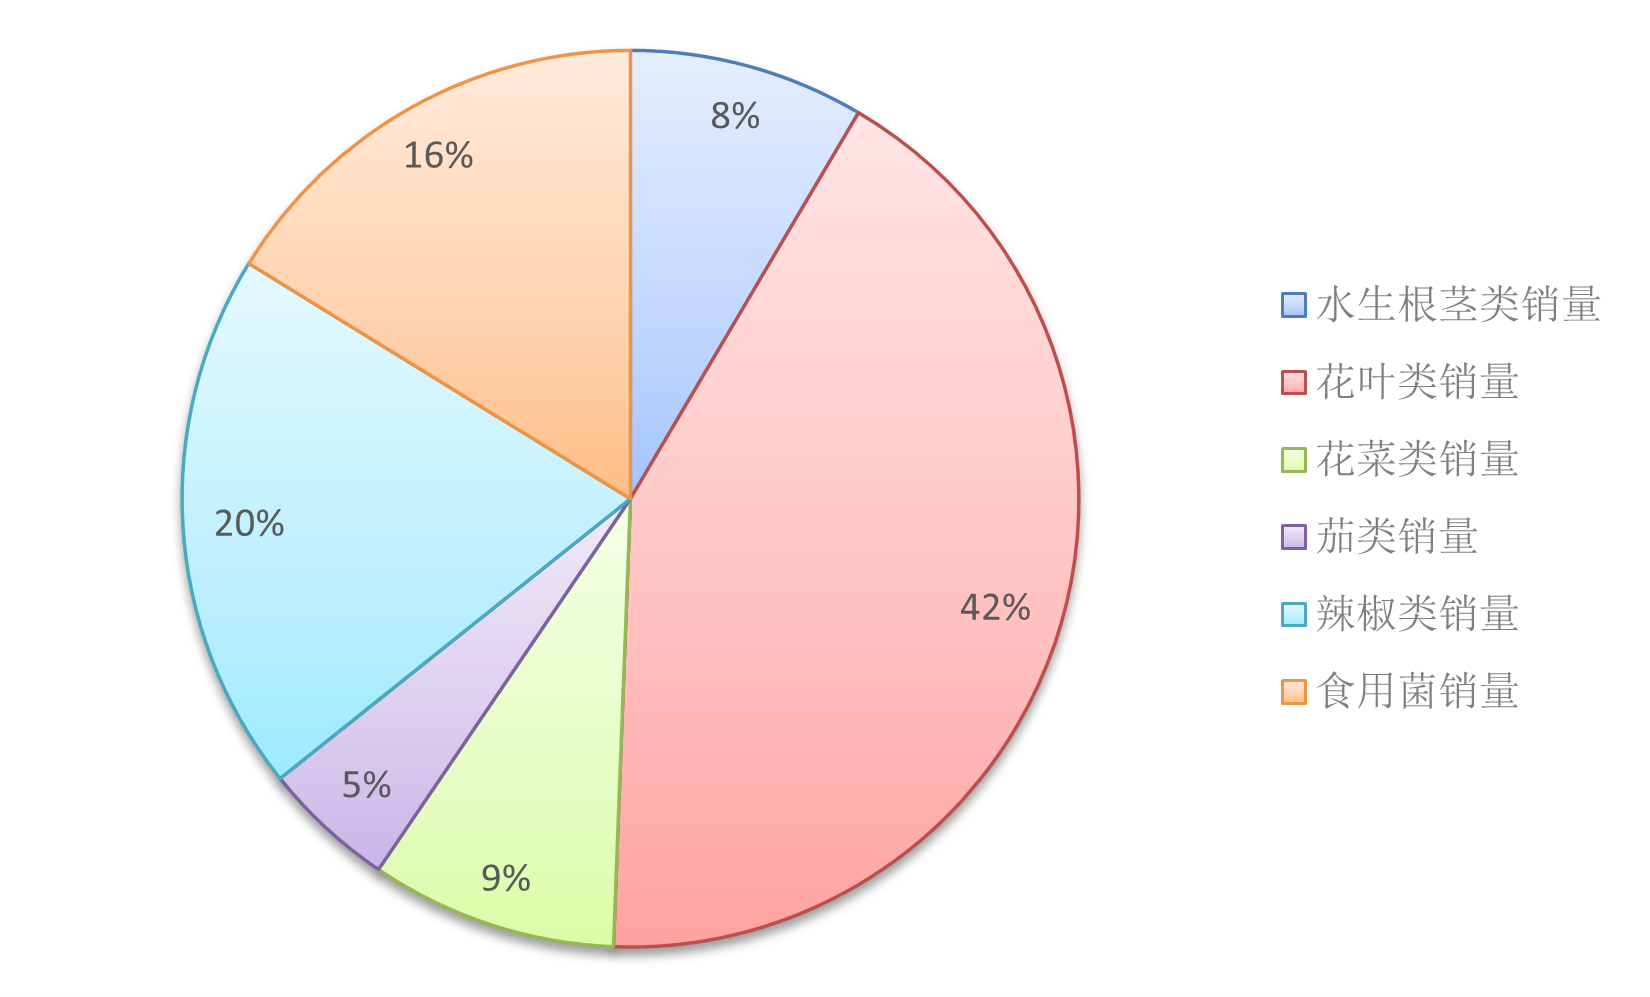
\includegraphics[width=.4\textwidth]{bilibili/template/figures/饼状图.png}%用width scale 还是height要根据图片选择
    \caption{描述性统计图}
    \label{描述性}%对应下文ref{}中的内容,编译为:引用“图1”
\end{figure}

\subsubsection{特征工程}
在数据预处理阶段,本研究采用了多种特征工程技术,旨在提升模型的准确性和解释性。以下是一些关键的操作和其对模型性能的潜在影响。

1.数据融合: 初始数据集被与其他相关数据表通过“单品编码”和“日期”等关键字段进行合并,这种方式可以丰富数据的维度,提供更多信息以供模型学习。

2.序号添加: 通过添加一个从1开始的序号列,为每一条记录赋予了唯一的标识,这样做有助于在后续的数据分析或模型验证中快速定位数据点。

3.时间特征提取: 
\begin{itemize}
    \item \textbf{星期}特征可揭示周期性购买行为。
    \item \textbf{年中进度}特征能够捕捉季节性效应。
    \item \textbf{周}, \textbf{月份}和\textbf{季度}特征为模型提供了不同的时间粒度,这有助于模型捕捉到在不同时间尺度上的规律。
    \item 将\textbf{扫码销售时间}转换为一天中的小数部分,可以更精细地描述时间信息。
\end{itemize}

4.特征转换:
\begin{itemize}
    \item  “交易金额”和“利润”通过现有的销量和价格信息计算得出,这两个特征可能是预测模型中的重要因素。
    \item  将“销售类型”和“是否打折销售”从文本转换为数值(1和-1,1和0),方便模型的数学处理。
\end{itemize}

5.数据规范化: 将“销售日期”转换回字符串格式,以统一数据类型。

这些特征工程步骤不仅提高了数据的多维度表达能力,也便于后续模型的学习与解释。例如,通过引入不同时间尺度的特征,模型能更好地学习和抓住时间序列中的潜在规律。此外,通过计算“交易金额”和“利润”,模型有机会学习到与目标变量更直接相关的特征,从而提高预测精度。总体而言,这一系列精心设计的特征工程步骤大大增强了数据集的信息密度和模型的预测能力。

\subsubsection{异常值处理}
\begin{figure}[H]%这用H,上方有float
	\centering
	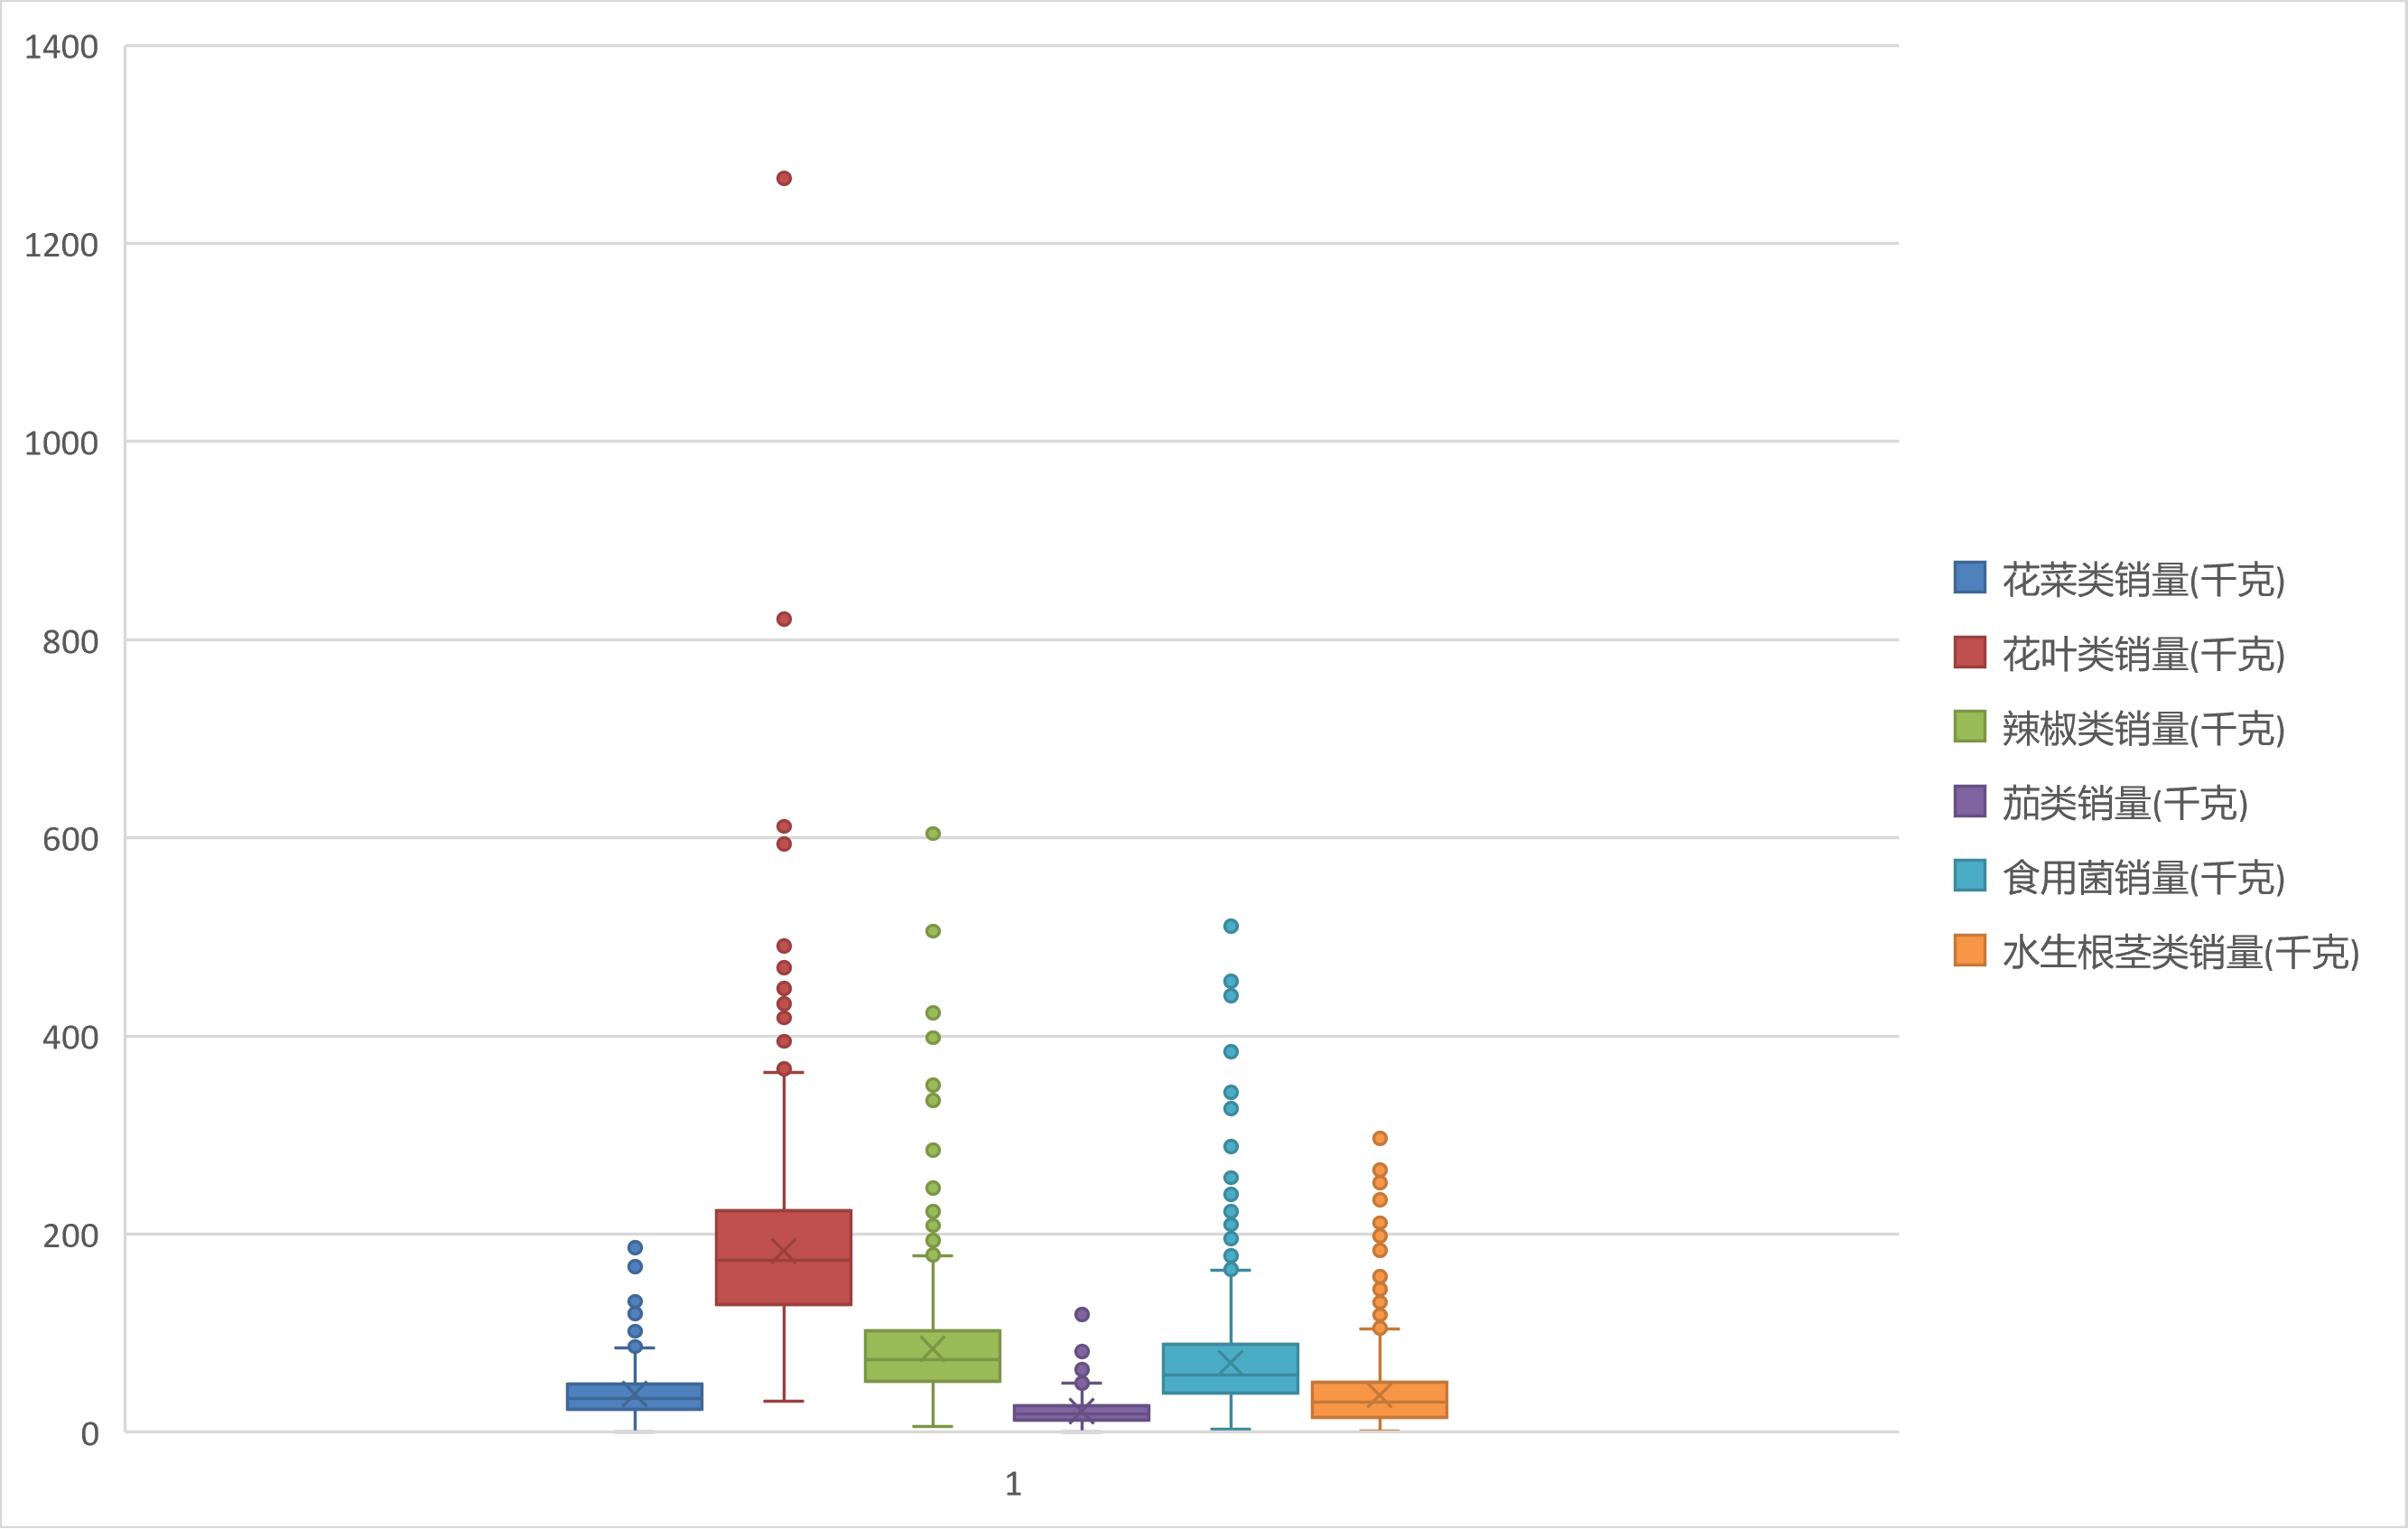
\includegraphics[width=0.6\textwidth]{bilibili/template/figures/箱线图.png}%用width scale 还是height要根据图片选择
    \caption{箱线图}
    \label{箱线图}%对应下文ref{}中的内容,编译为:引用“图1”
\end{figure}
分析销售数据常常需要处理可能导致统计度量偏斜的异常值或离群值。这些异常值可能由多种原因导致,例如数据录入错误、真实但极端的波动或者欺诈活动。识别并处理这些异常值对于从数据中获取准确的洞见至关重要。我们使用箱线图方法来检测“销量(千克)”中的异常值。计算该属性的第一四分位数(\( Q1 \))和第三四分位数(\( Q3 \))。然后确定上边缘(whisker)的极限值:
\[
\text{上边缘} = Q3 + 5 \times (Q3 - Q1)
\]
    
    如图\ref{箱线图}超过上限的即为异常值,这里,我们使用了5倍的四分位差,而非传统的1.5倍,以减少对异常值检测的敏感度。
在一个约束条件下进行异常值的替换:仅当异常值的数量少于总样本量的一定比例时才进行替换,这里的百分比设置为0.02(即2\%)。

替换策略与使用最近记录的平均值或中位数的传统方法有所不同。对于每一个检测到的异常值,我们识别相应的“单品名称”,找到所有具有相同单品名称的记录,计算这些记录的“销量(千克)”的平均值,并用其替换异常值。

\subsubsection{计算消除异常值}

\subsection{针对不同品类商品销售量分布规律可视化}
利用excel画出下述两张图:
\begin{figure}[H]%这用H,上方有float
	\centering
	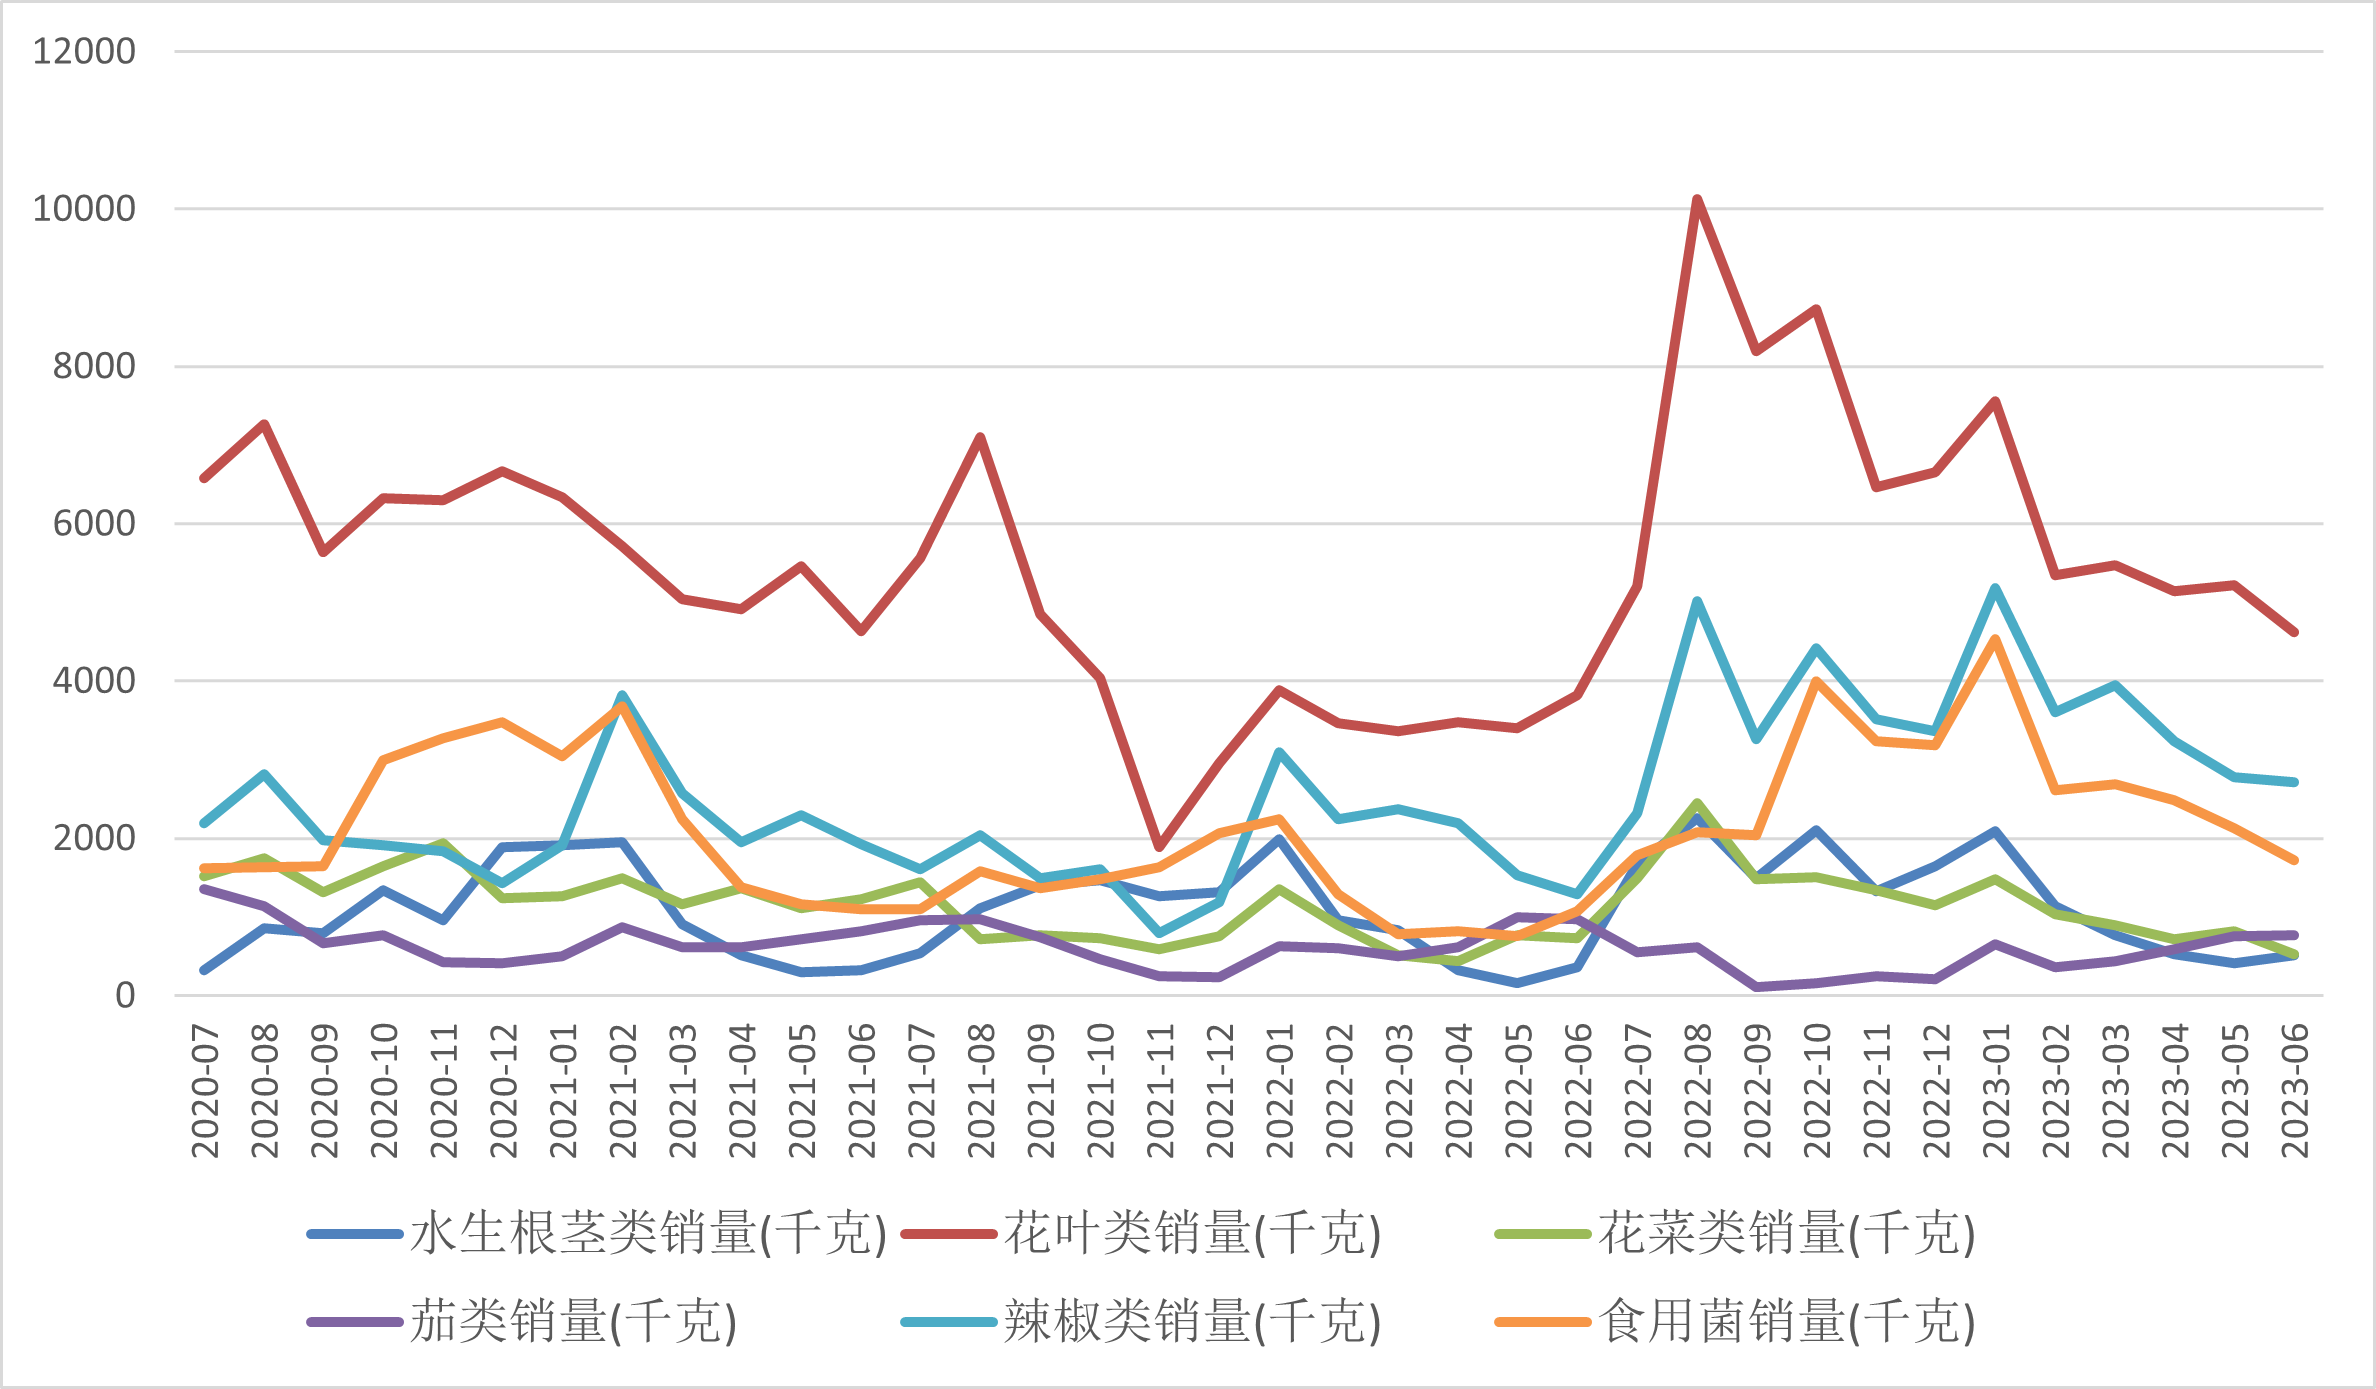
\includegraphics[width=0.6\textwidth]{bilibili/template/figures/品类的月分布规律.png}%用width scale 还是height要根据图片选择
    \caption{不同品类月销售量分布规律图}
    \label{不同品类分布规律图}%对应下文ref{}中的内容,编译为:引用“图1”
\end{figure}
由图\ref{不同品类分布规律图}可知,花叶类销量明显高于其他几类蔬菜类商品,说明花叶类的需求量最大。从分布规律也可知花叶、辣椒类、食用菌、水生根茎类商品在每年的6至8月的销售量基本呈上升趋势,且基本在8月达到最大值,说明供应量影响了分布规律。茄类商品的销量较低且几乎保持稳定,说明茄类的需求量较少,供给量也相对稳定。对于2022年8月至12月高于前后季度的现象,我们推测主要原因是供给量少,价格升高,销量减少:第一季度可能存在因疫情影响,出现的外省调入量小,供给量少;第二季度可能存在光照不足该省内蔬菜类商品供应量减少;第三季度可能恰逢省外蔬菜供应量增加;第四季度,受冷空气影响较大,供应量下降。


\subsection{不同品类日销售量的相关性分析}
\begin{figure}[H]%这用H,上方有float
	\centering
	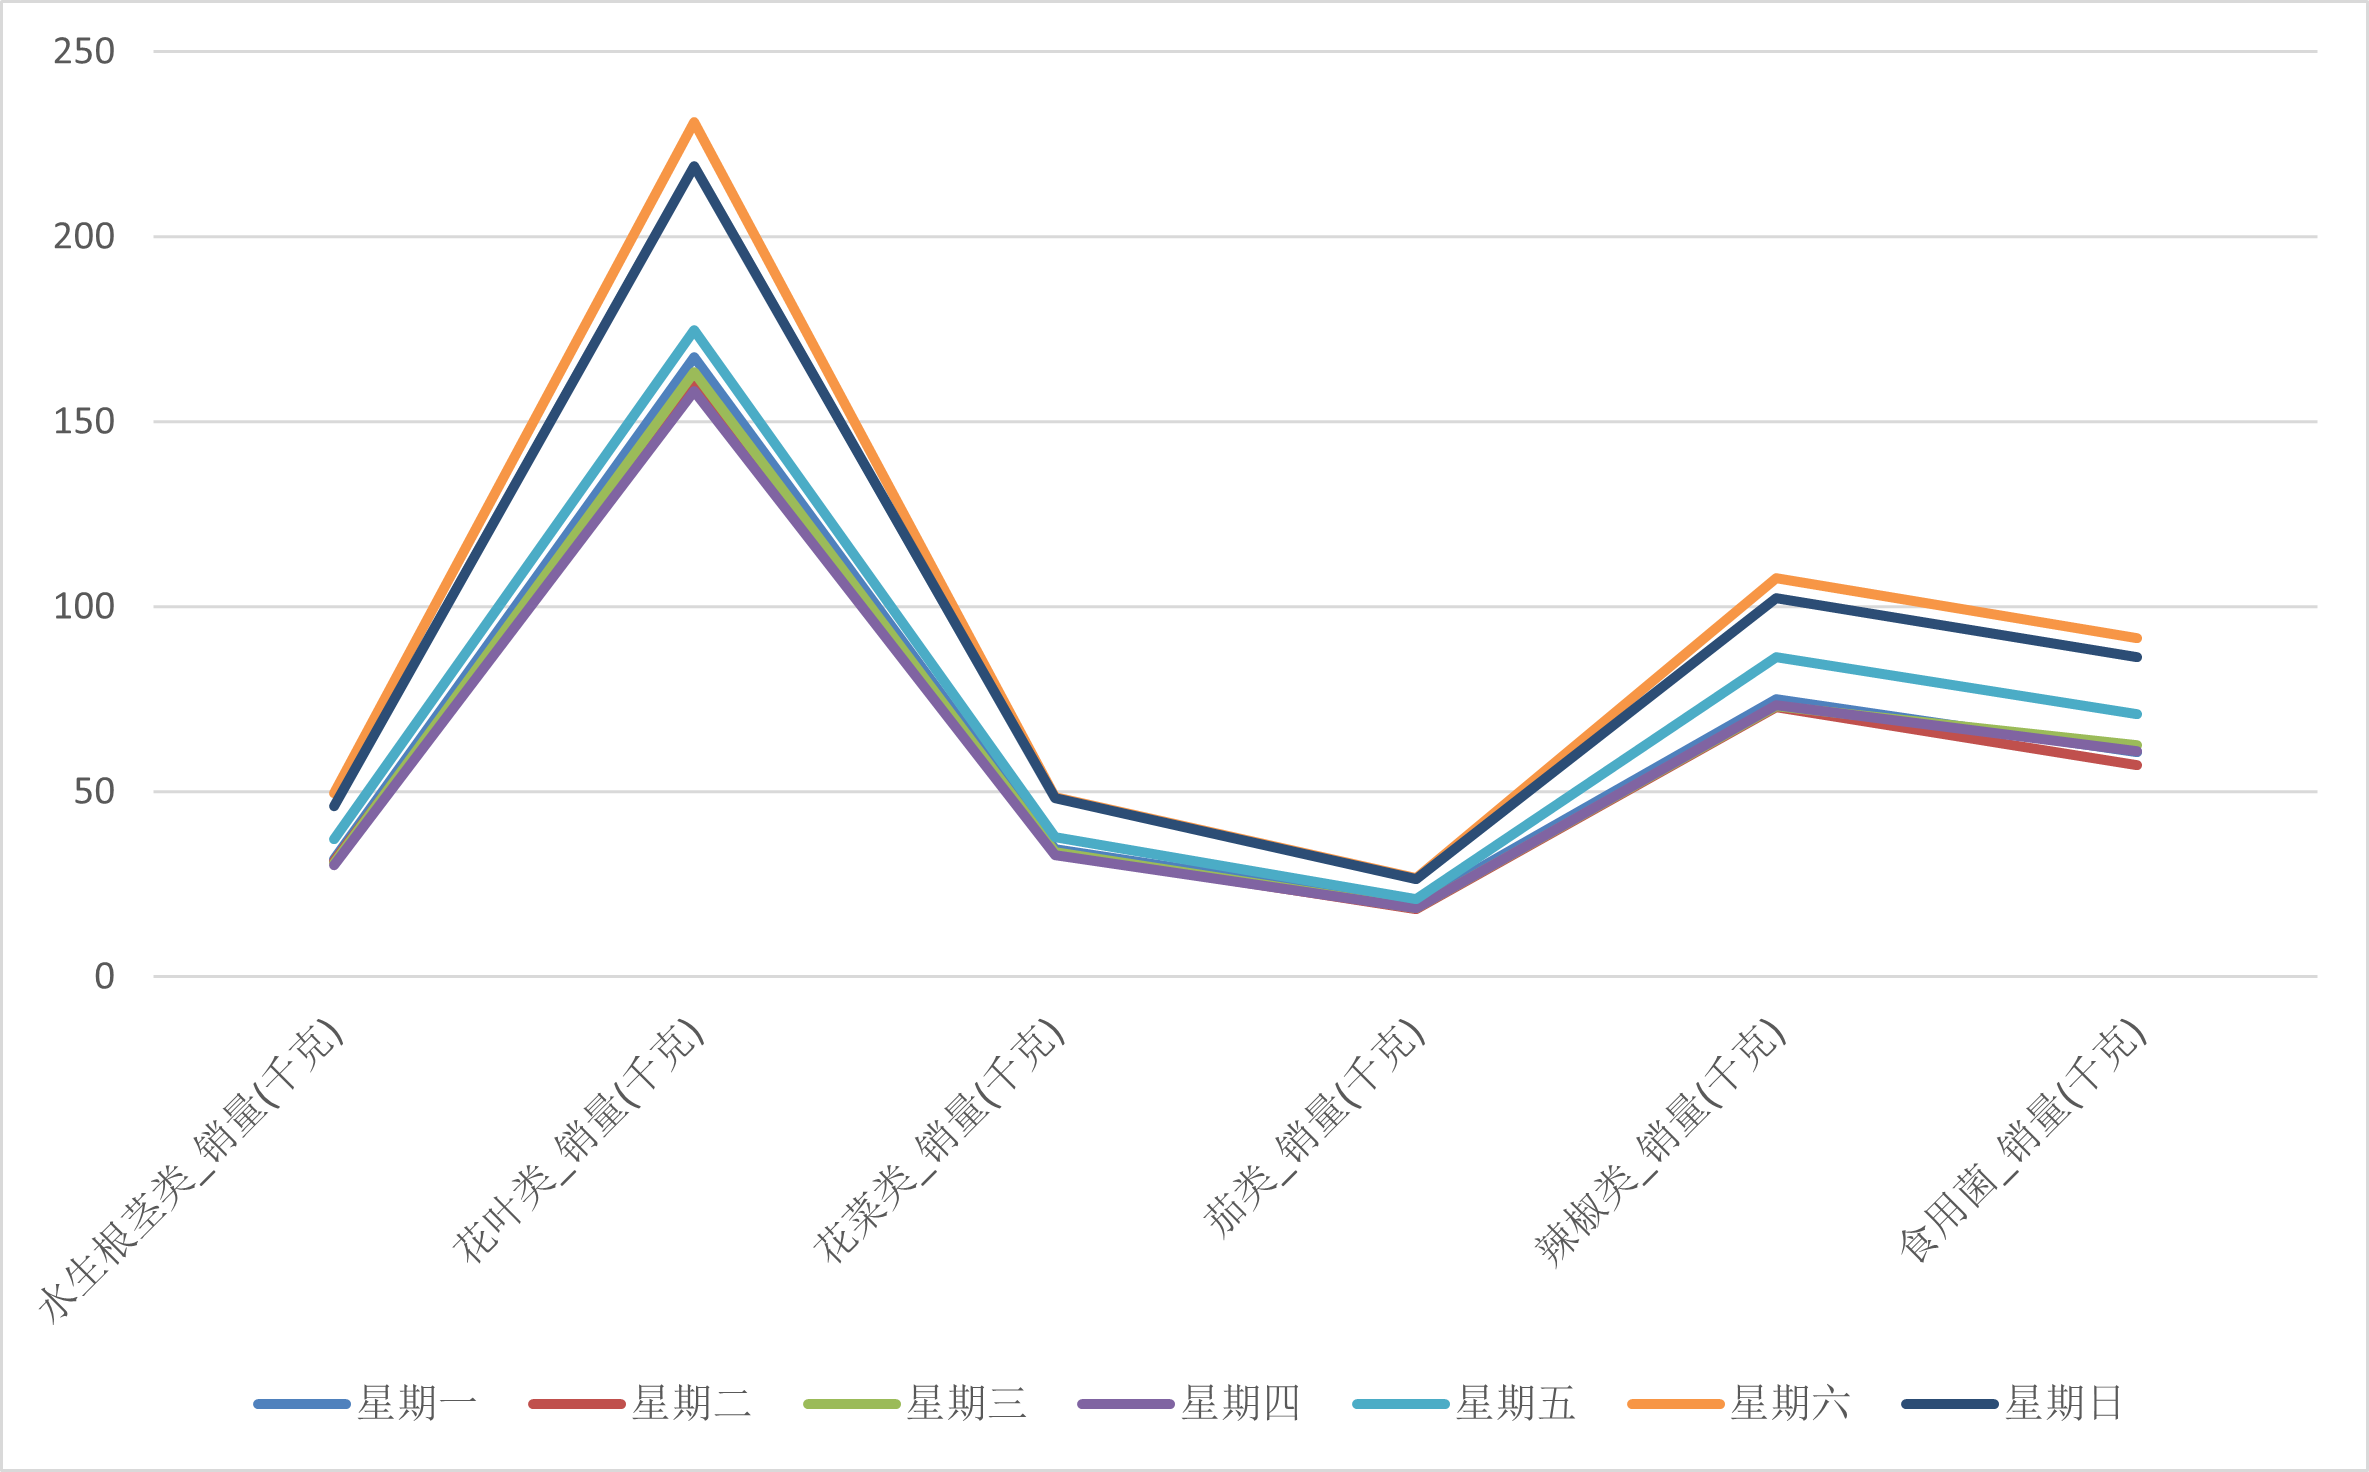
\includegraphics[width=0.6\textwidth]{bilibili/template/figures/品类的周内日销量.png}%用width scale 还是height要根据图片选择
    \caption{不同品类日销售量分布规律图}
    \label{日销量}%对应下文ref{}中的内容,编译为:引用“图1”
\end{figure}
由图\ref{日销量}可知,周末的蔬菜类商品销售量高于周中的商品销售量,说明一周内周末的蔬菜需求量较大。

\subsubsection{模型说明}
斯皮尔曼相关系数可用于测量两变量的关联程度,特别适用于非正态或有序数据。与基于原始数据的皮尔逊系数不同,它基于变量的排名进行计算,因此在处理非线性或单调关系时更鲁棒。系数范围为-1到1,接近1或-1表示强相关,0表示无相关。

\subsubsection{模型建立与求解}
首先,针对各类蔬菜的日销售量数据,我们执行Z-Score标准化以便将其转化为一个标准正态分布,该分布具有均值(μ)为0和标准差(σ)为1。这一步骤是为了消除不同量纲和数据分布的影响,从而使得数据更适于后续的统计分析或机器学习模型的应用。
\begin{equation}
	z_{i}=\dfrac{x_{i}-\mu }{\sigma }
\end{equation}
其中$z_{i}$表示标准化的值,$x_{i}$表示原始数据点,$\mu$表示数据的值,$\sigma$表示数据的标准差。

然后,基于Python计算Spearman相关系数矩阵。下述为其计算步骤(以花叶类和水生根茎类举例):
\begin{itemize}
\item 首先,对两个变量花叶类日销售总量$x$、水生根茎类日销售总量$y$的数据进行排名(等级分配)。
  
\item 计算排名差异(Rank Differences):对于每一对排名值($R_x$ 和 $R_y$),计算它们的差异($d_i = R_x - R_y$)。
  
\item 计算差异的平方和:将所有差异的平方和求和,得到一个值,表示排名之间的差异程度。
  
\item 计算斯皮尔曼相关系数 $\rho$(rho):使用以下公式计算斯皮尔曼
  相关系数:
 \begin{equation}
    \rho = 1 - \frac{6\sum d_i^2}{n(n^2 - 1)}
  \end{equation}
其中,$\rho$ 表示斯皮尔曼相关系数,$d_i$ 表示排名差异,$n$ 表示数据点的数量。
\end{itemize}
得到每日的Spearman相关系数矩阵热力图如下。
\begin{figure}[H]%这用H,上方有float
	\centering
	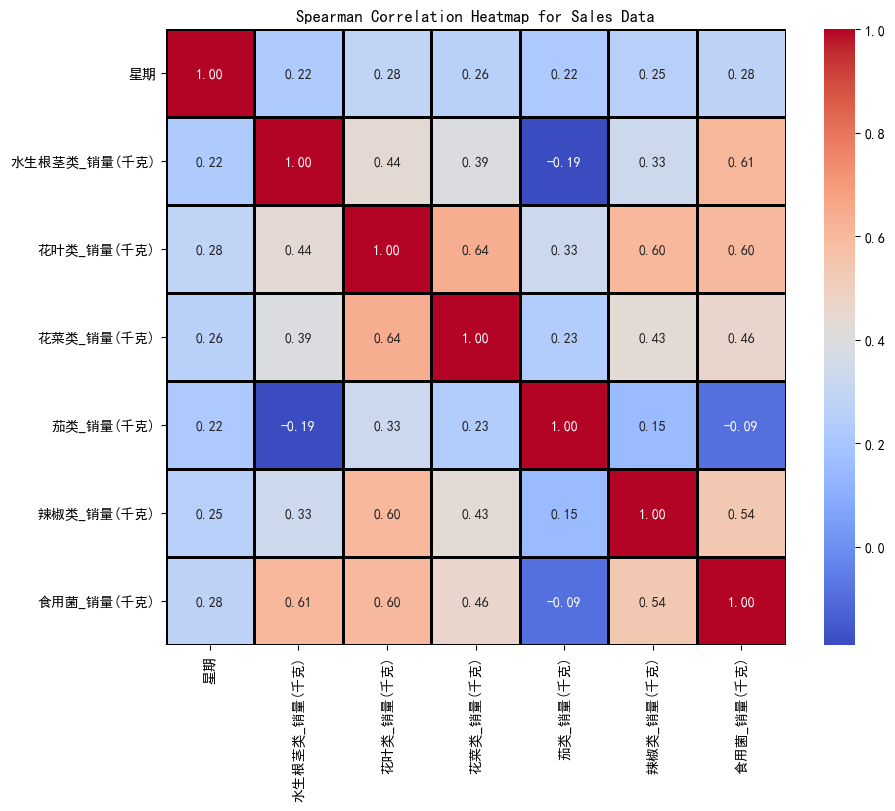
\includegraphics[width=0.55\textwidth]{bilibili/template/figures/日品类热力图.png}%用width scale 还是height要根据图片选择
    \caption{品类日销售量热力图}
    \label{日品类热力图}%对应下文ref{}中的内容,编译为:引用“图1”
\end{figure}
由图\ref{日品类热力图}可知,星期

\subsection{针对单品间的分布规律及相互关系}
\subsubsection{单品间的分布规律}
首先将各个蔬菜单品进行层次聚类得到图\ref{单品聚类图}。可以大致总结:大白菜为一类;净藕,芜湖青椒为一类;其他单品为一类。由此可见,白菜的需求量最高;净藕、青椒其次;其他类单品需求量较少。
\begin{figure}[H]%这用H,上方有float
	\centering
	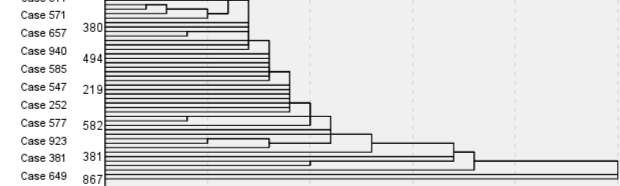
\includegraphics[width=0.8\textwidth]{bilibili/template/figures/聚类图1.png}%用width scale 还是height要根据图片选择
    \caption{单品聚类图(部分)}
    \label{单品聚类图}%对应下文ref{}中的内容,编译为:引用“图1”
\end{figure}
用excel分别绘制大白菜分布规律图,和其他类别中抽选保康高山大白菜分布规律图;再绘制第二类中的芜湖青椒和净藕分布规律图。
\begin{figure}[H]%这用H,上方有float
	\centering
	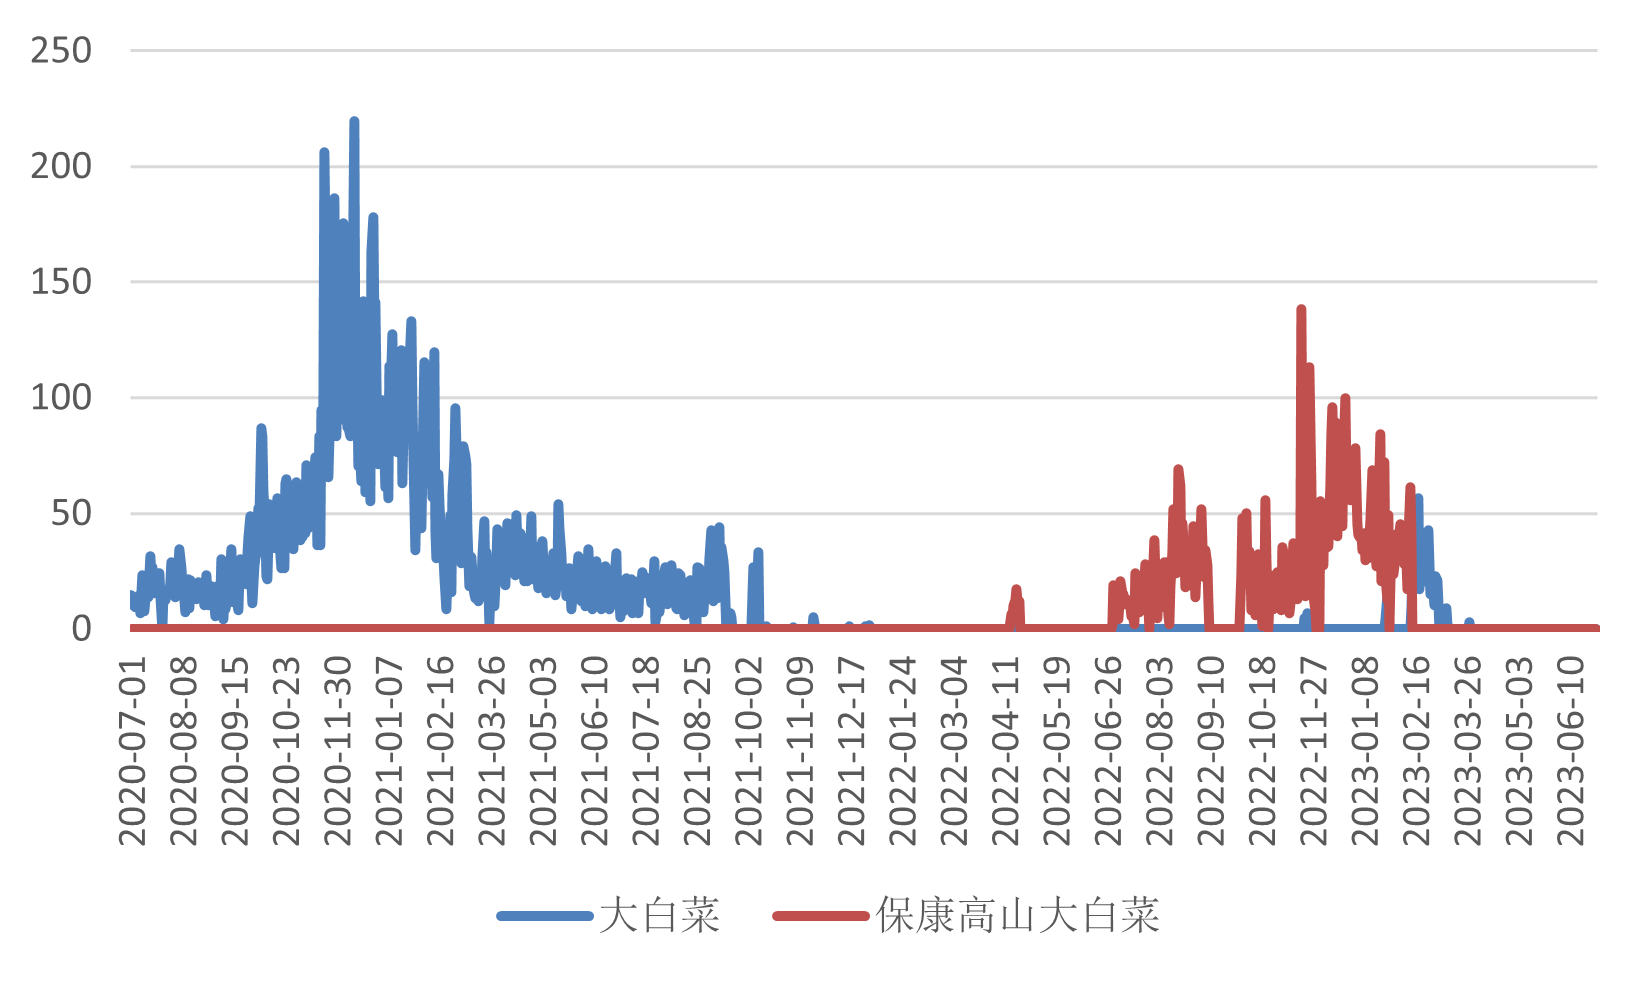
\includegraphics[width=0.6\textwidth]{bilibili/template/figures/聚类13单品图.png}%用width scale 还是height要根据图片选择
    \caption{第一、三类单品分布规律图}
    \label{聚类1图}%对应下文ref{}中的内容,编译为:引用“图1”
\end{figure}
\begin{figure}[H]%这用H,上方有float
	\centering
	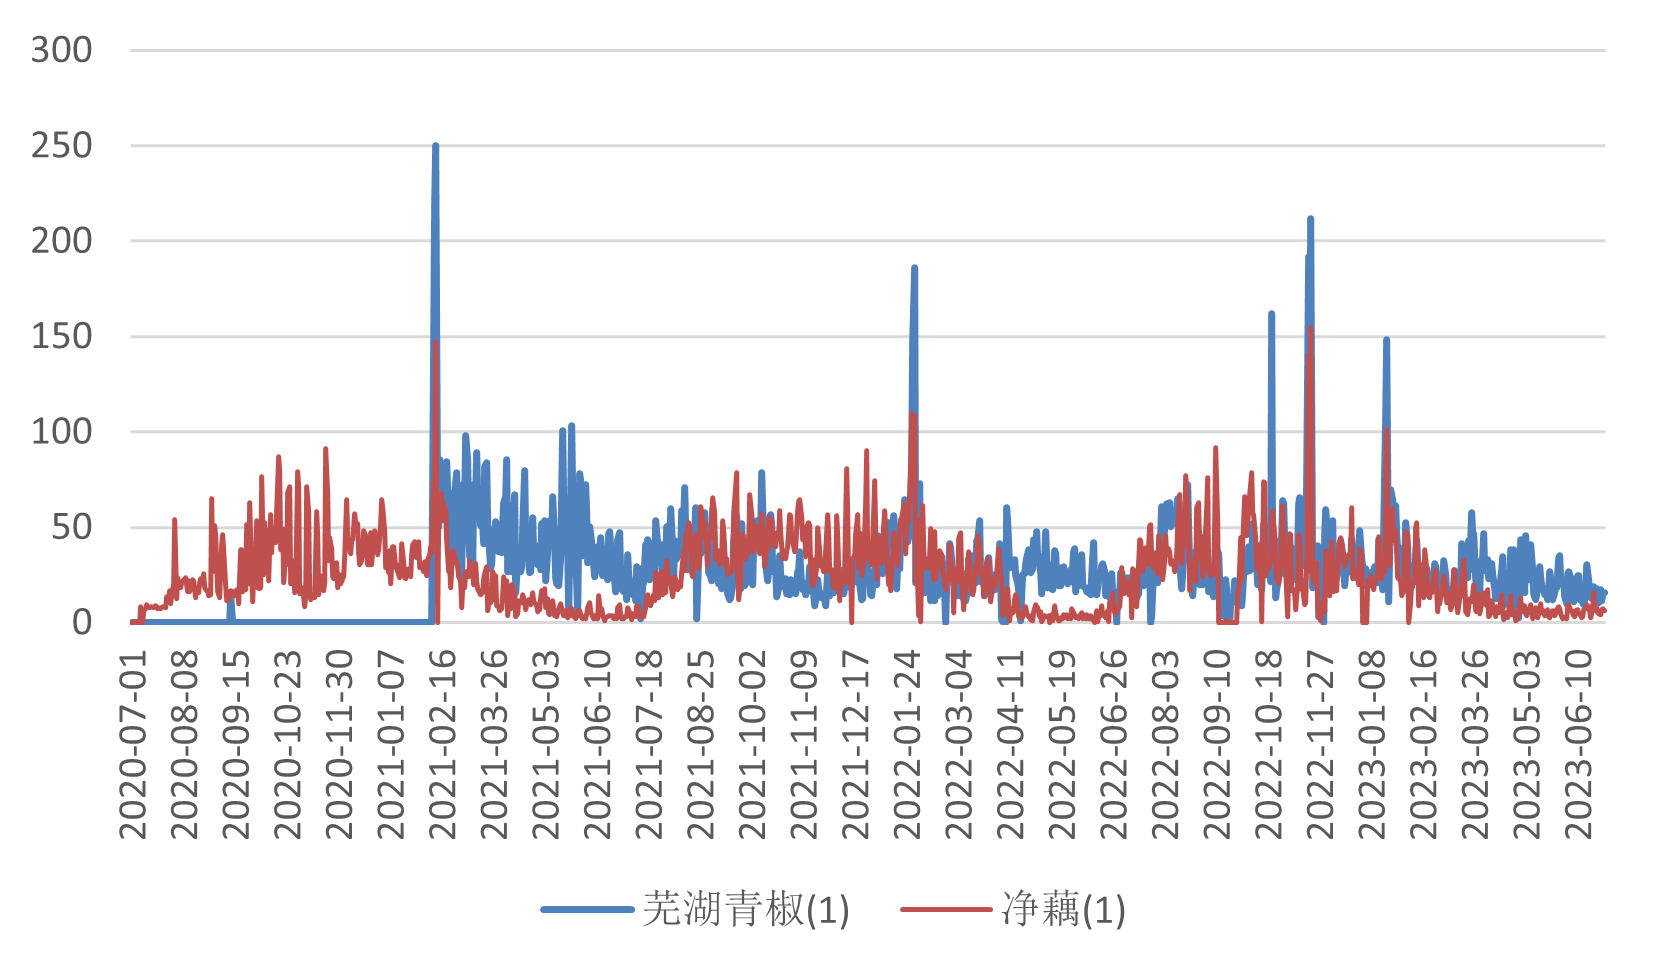
\includegraphics[width=0.6\textwidth]{bilibili/template/figures/聚类2单品图.png}%用width scale 还是height要根据图片选择
    \caption{第二类单品分布规律图}
    \label{聚类2图}%对应下文ref{}中的内容,编译为:引用“图1”
\end{figure} 
由图\ref{聚类1图}可知大白菜在2020年至2021年中供货量较多,后期推测被保康高山大白菜等单品其他类的单品代替。经网上查阅资料显示,高山大白菜的营养价值更高,推测消费者对身体健康等生活质量水平要求提升。由图\ref{聚类2图}可知其芜湖青椒与净藕的分布规律基本相同。

\subsubsection{单品间的相关性分析}
蔬菜各单品间的模型建立和求解过程与上文蔬菜品类间的过程类似,在次不过多赘述。
\begin{figure}[H]%这用H,上方有float
	\centering
	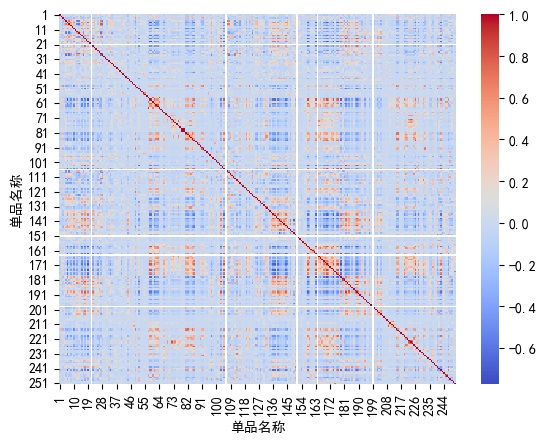
\includegraphics[width=0.6\textwidth]{bilibili/template/单品相关性分析.png}%用width scale 还是height要根据图片选择
    \caption{单品相关性销售量热力图}
    \label{单品相关性销售热力图}%对应下文ref{}中的内容,编译为:引用“图1”
\end{figure}
由图\ref{单品相关性销售热力图}可知单品相关性的强弱,我们抽取其中几种特殊的单品数据进行定性分析。

在蔬菜单品之间,存在两种主要的相关性:正相关性和负相关性。正相关性,也可被称为互补关系,指的是当消费者购买某一种蔬菜单品时,有高概率同时购买另一种单品。
\begin{table}[H]
	\centering
	\caption{单品正相关性表}
	\label{单品正相关性表}
	\begin{tabular}{ccc}
		\toprule[1.5pt]
		\makebox[0.25\textwidth][c]{单品名称}	&  \makebox[0.25\textwidth][c]{单品名称2}&
        \makebox[0.25\textwidth][c]{斯皮尔曼系数}\\ 
		\midrule[1pt]		
大白菜  & 金针菇          & 0.858  \\
螺丝椒  & 姜蒜小米椒组合装(小份) & 0.864 \\
\bottomrule[1.5pt]		
	\end{tabular}
\end{table}
由表\ref{单品正相关性表}可知呈现较强正相关性的情况大多与做菜时的配菜习惯有关,例如常作为火锅涮菜的金针菇和大白菜;作为佐料的辣椒类单品可能会同时购买多种等情况。


反之,负相关性,也可称为替代关系,意味着消费者在购买某一单品后,很可能会避免购买某种其他单品,展示出“此消彼长”的现象。
\begin{table}[H]
	\centering
	\caption{单品负相关性表}
	\label{单品负相关性表}
	\begin{tabular}{ccc}
		\toprule[1.5pt]
		\makebox[0.25\textwidth][c]{单品名称}	&  \makebox[0.25\textwidth][c]{单品名称2}&
        \makebox[0.25\textwidth][c]{斯皮尔曼系数}\\ 
		\midrule[1pt]		
云南油麦菜 & 云南油麦菜(份) & -0.773 \\
云南油麦菜 & 云南生菜(份)  & -0.745 \\
云南油麦菜 & 螺丝椒(份)   & -0.734\\
\bottomrule[1.5pt]		
	\end{tabular}
\end{table}
由表\ref{单品负相关性表}可知呈现较强负相关性的情况大致有三种:(1)同种单品,但是售卖方式不同;例如是否按份卖的油麦菜。(2)两种相似单品,购买其中一种,另一种会减少;譬如油麦菜与生菜一般消费者会选择其中一种青菜。(3)做菜习惯,菜品搭配引起的;例如油麦菜一般清炒而非与螺丝椒搭配。

\begin{table}[H]
	\centering
	\caption{单品特殊情况表}
	\label{单品特殊情况表}
	\begin{tabular}{ccc}
		\toprule[1.5pt]
		\makebox[0.25\textwidth][c]{单品名称}	&  \makebox[0.25\textwidth][c]{单品名称2}&
        \makebox[0.25\textwidth][c]{斯皮尔曼系数}\\ 
		\midrule[1pt]		
        红珊瑚(粗叶) & 红橡叶   & 1      \\
        红珊瑚(粗叶) & 绿牛油   & 1      \\
        红橡叶     & 绿牛油   & 1   \\
		\bottomrule[1.5pt]		
	\end{tabular}
\end{table}
我们发现有三对变量斯皮尔曼的相关系数为1,如上表\ref{单品特殊情况表}呈现。针对此特殊情况,我们对excel中的数据进行了筛选,发现红珊瑚、红橡叶、绿牛油都仅购买了一次。并且经过网上查阅资料可得,该三种单品都可用来制作沙拉等轻食。此类蔬菜单品为特殊情况。



\section{问题二}
\subsection{利用CRITIC权重法计算各品类批发价格}
\subsubsection{模型的建立}
CRITIC是一种多准则决策分析方法,用于确定各个准则(或特征)的权重。这种方法主要适用于那些需要在多个相互竞争的准则下做出决策的情况,而由第一问相关性可知蔬菜各单类间大多正符合这样的竞争关系。其中涉及到的重要公式如下:
(1)计算指标变异量
\begin{equation}
\sigma_j = \sqrt{\frac{1}{n} \sum_{i=1}^n (x_{ij} - \bar{x}_j)^2}
\end{equation}
$\sigma_j$为第j个指标的标准差,n为单品的数量,$x_ij$为第i个样本在第j个指标上的取值,$\bar{x}_j$为第j个指标的平均值。

(2)计算指标冲突
\begin{equation}
r_{jk} = \frac{\sum_{i=1}^n (x_{ij} - \bar{x}_j)(x_{ik} - \bar{x}_k)}{\sqrt{\sum_{i=1}^n (x_{ij} - \bar{x}_j)^2 \sum_{i=1}^n (x_{ik} - \bar{x}_k)^2}}
\end{equation}
其中$r_jk$为第j个和第k个指标之间的相关系数,用以衡量两个指标的冲突性。

(3)计算其信息量
\begin{equation}
c_j = \sigma_j \times (1 - \sum_{k=1, k \neq j}^m |r_{jk}|)
\end{equation}
其中$c_j$为信息量,m是属性的数量。

(4)计算其属性权重
\begin{equation}
w_j = \frac{c_j}{\sum_{j=1}^m c_j}
\end{equation}
其中$w_j$为属性权重。

(5)某蔬菜品类的批发价格
\begin{equation}
C_{\text {类 }}=\sum_{j=1}^{n} w_{j} \times C_{\text {单 }}
\end{equation}
其中$C_{\text {类 }}$为该品类的批发价格,$C_{\text {单 }}$为该单品的批发价格。
\subsubsection{模型的求解}
借助Python求解,并将其权重值降序排列,表\ref{权重表}展示一部分结果,发现其权重值与第一问的聚类结果基本相同,说明销量大的单品对品类的批发价影响越大,同时可验证该方法计算权重具有客观性。
\begin{table}[H]
	\centering
	\caption{权重表(部分)}
	\label{权重表}
	\begin{tabular}{ccccc}
 \toprule[1.5pt]
		\makebox[0.2\textwidth][c]{单品名称}	&  \makebox[0.2\textwidth][c]{指标冲突}&
        \makebox[0.2\textwidth][c]{信息量}&
        \makebox[0.2\textwidth][c]{权重}\\ 
		\midrule[1pt]	
 大白菜     & 242.259 & 7419.788 & 4.15  \\
金针菇(盒)  & 232.148 & 6346.543 & 3.549 \\
芜湖青椒(1) & 229.375 & 5622.615 & 3.145 \\
云南生菜(份) & 233.200 & 5246.724 & 2.934 \\
泡泡椒(精品) & 243.962 & 4779.878 & 2.673\\
\bottomrule[1.5pt]		
	\end{tabular}
\end{table}
利用权重可进一步将品类的进货价格计算得出,数据于支撑材料中展出。


\subsubsection{模型的建立}



\subsection{针对销售总量与成本加成
定价的关系}
\subsubsection{成本加成定价的定义}
成本加成定价的基本思想是首先确定产品或服务的生产成本,然后在这个成本的基础上加上一个利润率来确定最终的销售价格。
首先确定成本加成定价的计算公式\cite{成本加成定价法评介}:
\begin{align}
  M=\dfrac{C-W}{W}\\
  P=W\times \left( 1+M\right)
\end{align}
其中P为成本加成定价,C为售价,W为进货成本,M为成本加成率。
\subsubsection{相关性的研究}

利用Python求出Spearman的系数矩阵如图\ref{成本定价相关性},可知各个单品类销量与成本加成定价相关性系数基本为0,相关性不大。
\begin{figure}[H]%这用H,上方有float
	\centering
	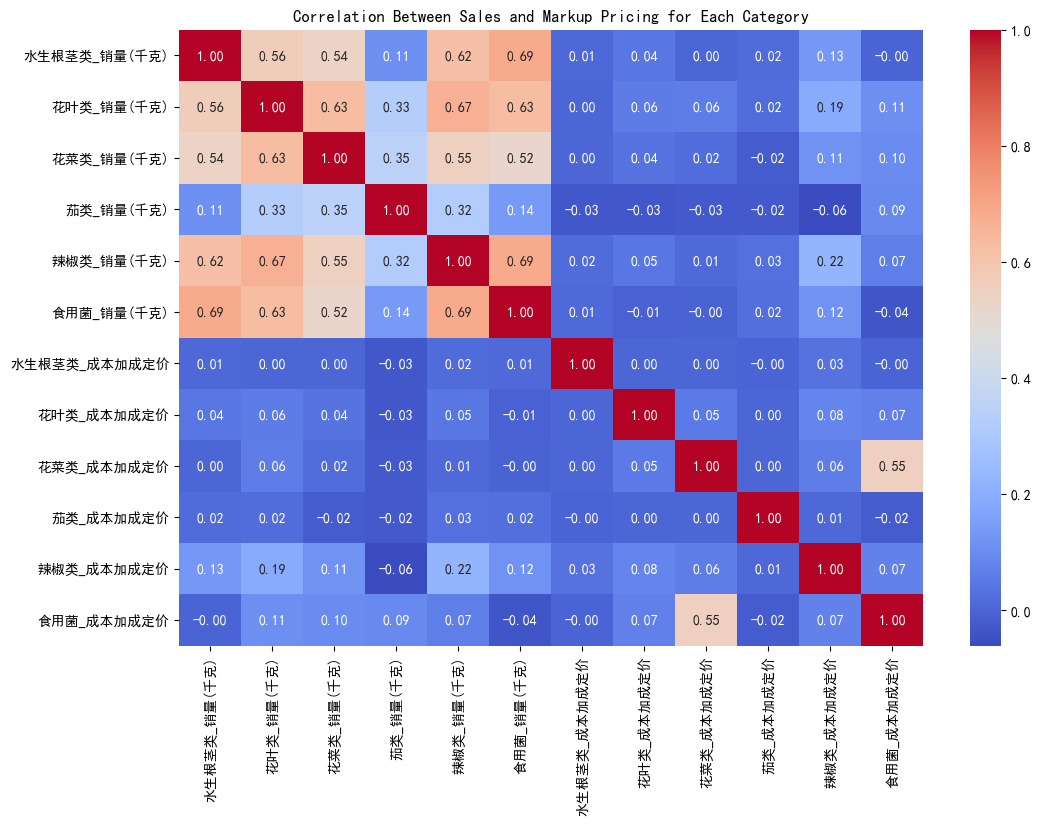
\includegraphics[width=.75\textwidth]{bilibili/template/figures/成本定价相关性分析.png}%用width scale 还是height要根据图片选择
    \caption{成本定价相关性}
    \label{成本定价相关性}%对应下文ref{}中的内容,编译为:引用“图1”
\end{figure}

在此之上,我们尝试了多种回归模型,以水生根茎类单品的线性回归模型为例,由表\ref{2}可知拟合值为0.066,远小于1,拟合程度程度不高。
\begin{table}[H]
	\centering
	\caption{线性回归模型结果}
	\label{2}
	\begin{tabular}{ccc}
		\toprule[1.5pt]
		\makebox[0.3\textwidth][c]{单品名称}	& 
        \makebox[0.4\textwidth][c]{方程} &
       \makebox[0.3\textwidth][c]{$R_{2}$} \\ 
		\midrule[1pt]		
		水生根茎类& \( y = 63.686 - 0.541x \) & 0.066	\\
		\bottomrule[1.5pt]		
	\end{tabular}
\end{table}




\subsection{预测模型}

\subsection{prophet预测模型}
\subsubsection{模型的建立}
Prophet预测模型是基于时间序列分解和机器学习拟合的时间序列预测的模型。
由第一问的数据处理及分布规律本研究中的蔬菜商品数据存在强季节性影响和部分缺失的特点,非常适用该模型。Prophet将时间序列分解为三个主要组件:趋势、季节性和节假日效应。
数学上,Prophet模型可以表示为:
\begin{equation}
y(t) = g(t) + s(t) + h(t) + \epsilon_t
\end{equation}
其中y(t)是成本加成定价、销售总量在时间t的观察值,g(t)表示时间序列在非周期上面的变化趋势;s(t)表示周期项,或者称为季节项;h(t)表示节假日项,本研究设置的是春节、中秋节、国庆。$\epsilon_t$是误差项。

利用prophet模型预测品类补货量的数值(表\ref{table}所示)和品类加权后的成本加成利润率值如表\ref{table1}所示。

\subsubsection{模型的求解}


\begin{longtable}{ccccccc}
	\caption{品类补货总量预测结果表}
	\label{table}\\
		\toprule[1.5pt]
  日期    & 水生根茎类  & 花叶类    & 花菜类    & 茄类     & 辣椒类    & 食用菌    \\
  \midrule[1pt]
  \endfirsthead
7月1日        & 38.3468        & 197.9971     & 41.51457     & 39.91364    & 92.35294     & 84.94975     \\
7月2日        & 36.86538       & 191.9052     & 41.91052     & 39.82326    & 88.93235     & 82.37727     \\
7月3日        & 30.24122       & 166.2229     & 35.3         & 36.36012    & 75.38535     & 70.10578     \\
7月4日        & 30.272         & 162.5733     & 34.87396     & 35.60863    & 73.68088     & 68.30854     \\
7月5日        & 30.12657       & 164.2203     & 35.19643     & 35.33275    & 72.93051     & 71.1862      \\
7月6日        & 30.9091        & 162.7049     & 35.35139     & 35.51287    & 73.87488     & 71.49922     \\
7月7日        & 34.61324       & 171.2374     & 38.01292     & 36.50903    & 79.63304     & 76.77574\\
\bottomrule[1.5pt]
	\end{longtable}


\begin{longtable}{ccccccc}
	\caption{品类批发价格预测结果表}
	\label{table1}\\
		\toprule[1.5pt]
 日期   & 水生根茎类  & 花叶类     & 花菜类    & 茄类     & 辣椒类    & 食用菌    \\
  \midrule[1pt]
  \endfirsthead
7月1日 & 8.197178 & 3.595441 & 9.043356 & 3.499471 & 4.391681 & 4.633959 \\
7月2日 & 7.868449 & 3.64171  & 9.077476 & 3.497701 & 4.465746 & 4.640883 \\
7月3日 & 7.566247 & 3.62565  & 9.130813 & 3.400104 & 4.490141 & 4.790551 \\
7月4日 & 7.210955 & 3.626866 & 9.118385 & 3.308526 & 4.570404 & 4.762298 \\
7月5日 & 6.933749 & 3.680391 & 9.151319 & 3.291126 & 4.667824 & 4.774939 \\
7月6日 & 6.471597 & 3.646673 & 9.203922 & 3.248276 & 4.74194  & 4.843018 \\
7月7日 & 6.109254 & 3.632791 & 9.250042 & 3.180142 & 4.870018 & 4.833927\\
\bottomrule[1.5pt]
	\end{longtable}

\subsubsection{绘制预测图}
 图\ref{diaoduhou1}中左侧为水生根茎类的销售总量预测图,右侧为水生根茎类的成本加成利润率预测图黑色表示原始的时间序列离散点,深蓝色的线表示使用时间序列来拟合所得到的取值,而浅蓝色的线表示时间序列的一个置信区间。同时,可发现销售总量受节假日因素影响较大,可知节假日需求量大。并且,可知成本加成利润率基本稳定。
\begin{figure}[H]
	\caption{预测示意图}
	\label{diaoduhou1}
	\subfigure
	{
		\begin{minipage}[b]{.3\linewidth}
			\centering
			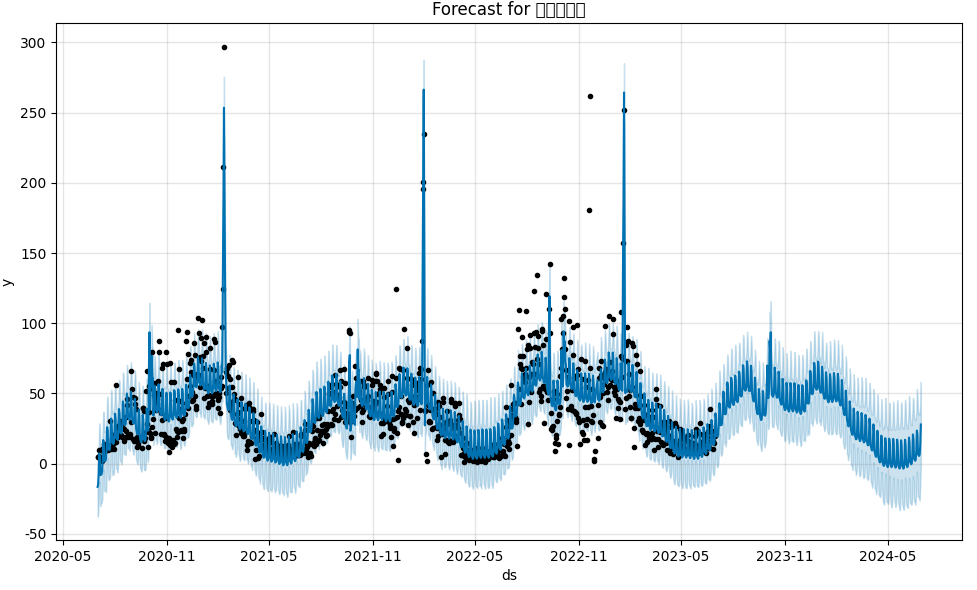
\includegraphics[scale=0.3]{bilibili/template/figures/根茎时间预测.png}
		\end{minipage}
	} \quad \quad \quad \quad\quad\quad
	\subfigure
	{
		\begin{minipage}[b]{.3\linewidth}
			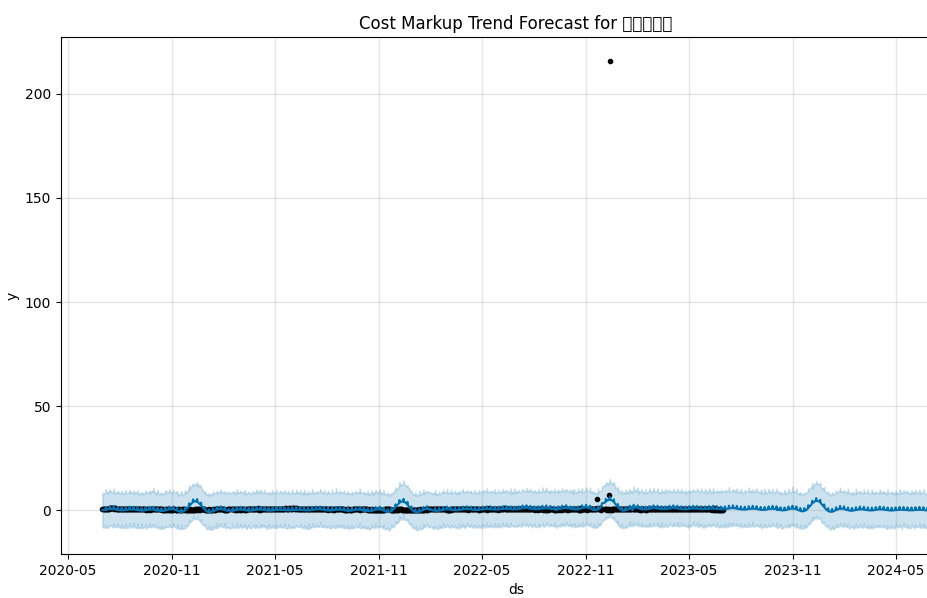
\includegraphics[scale=0.3]{bilibili/template/figures/水生根茎类成本加成利润率预测.png}
   
		\end{minipage}
	}
 \end{figure}
同时还可绘制出图,预测未来7天的批发价格,用于之后优化模型的建立。
\begin{figure}[H]%这用H,上方有float
	\centering
	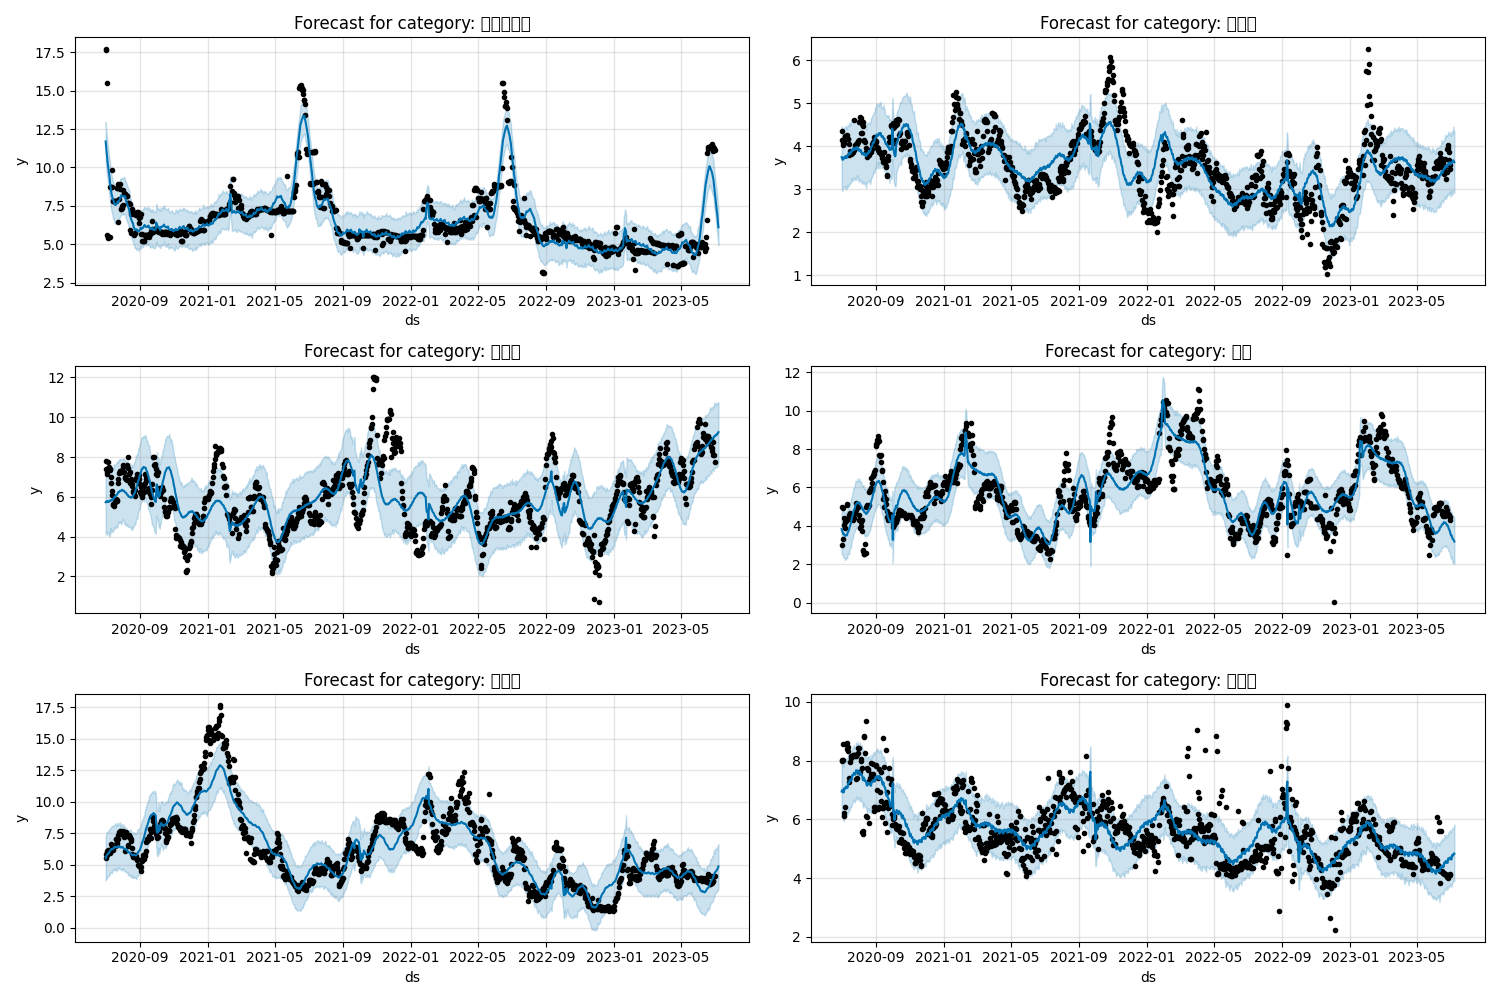
\includegraphics[width=0.8\textwidth]{bilibili/template/figures/批发价格预测图.png}%用width scale 还是height要根据图片选择
    \caption{品类批发价格预测图}
    \label{批发}%对应下文ref{}中的内容,编译为:引用“图1”
\end{figure}

\subsection{神经网络推算其最优值}
\subsubsection{模型的建立}
设 \( P_{mr} \) 为标价率(Mark-up Ratio),\( Q_{\text{in}} \) 为每个蔬菜类别的库存量。\( M \) 表示批发价格,\( \lambda \) 表示衰减率,\( S \) 表示销售预测。最大化利润的目标函数定义为:
\begin{equation}
\text{利润} = R - L - S - \text{惩罚项}
\end{equation}

其中,

\begin{align*}
  R = \sum_{i} C_i \times Q_{\text{out},i}   
\end{align*}
\begin{align*}
L = \sum_{i} \lambda_i \times M_i \times Q_{\text{in},i} 
\end{align*}
\begin{align*}
    S = \sum_{i} M_i \times Q_{\text{in},i} 
\end{align*}
\begin{align*}
C = M \times (1 + P_{mr}) 
\end{align*}
\begin{align*}
Q_{\text{out}} = (1 - \lambda) \times Q_{\text{in}} 
\end{align*}
\begin{align*}
\text{惩罚项} = \alpha \sum_{i} (C_i - C_{\text{目标},i})^2 + \beta \sum_{i} (Q_{\text{in},i} - Q_{\text{in, 目标},i})^2
\end{align*}

这里\( C_{\text{目标}} \) 和 \( Q_{\text{in, 目标}} \) 分别是成本和库存水平的目标值。\( \alpha \) 和 \( \beta \) 是惩罚系数。

其中优化的约束条件定义为:

\[
\begin{aligned}
P_{mr\text{下界},i} \leq P_{mri} \leq P_{mr\text{上界},i} \\
\end{aligned}
\]

其中 \( P_{mr\text{下界}} \) 和 \( P_{mr\text{上界}} \) 是标价率 \( P \) 的类别特定的下界和上界。
\subsubsection{模型的求解}
优化问题使用 Python 中的 \texttt{scipy.optimize.minimize} 函数通过顺序二次规划(SQP)方法进行求解,可得以下结果(顺序依次对应水生根茎类,花叶类,花菜类,茄类,辣椒类,食用菌):
\begin{itemize}
  \item 优化后的 \( P \) 值:[0.8184, 0.6366, 0.6533, 1.9028, 0.7914, 0.4578]
    \item 优化后的 \( Q_{\text{in}} \) 值:[40.85, 176.55, 42.98, 50.75, 85.68, 77.71]
    \item 最大化的利润:853.16(元/天)
\end{itemize}


\subsection{调度方案灵敏性与敏感性分析}

\section{问题三}
\subsection{模型建立}

\subsubsection{目标函数}
目标是最大化超市的收入,收入计算公式如下:
\[
\text{Revenue} = \sum \left( \text{预测销量} \times \text{预测价格} \times \text{预测利润率} \times \left(1 - \frac{\text{损耗率(\%)}}{100}\right) \right)
\]

\subsubsection{约束条件}

\begin{itemize}
    \item 可售单品总数必须控制在 \textbf{27-33} 个:通过灰狼优化算法中的 \texttt{lower\_bound} 和 \texttt{upper\_bound} 参数来实现的。
    \item 各单品订购量必须满足最小陈列量 \textbf{2.5千克} 的要求:在目标函数中,我们添加了一个惩罚项来处理这个约束。
\end{itemize}

具体来说,惩罚项的形式如下:
\[
\text{Penalty\_display} = \lambda_{\text{penalty}} \times \left( \text{min\_display\_weight} - \text{预测销量} \right)^2 \times I\left( \text{预测销量} < \text{min\_display\_weight} \right)
\]
其中,\( I() \) 是一个指示函数,当预测销量小于最小陈列量时取值为 1,否则为 0。


\subsubsection{惩罚函数}
为了确保满足约束条件,我们在目标函数中加入了一个惩罚项。对于不满足最小陈列量要求的单品,惩罚函数为:
\[
\text{penalty\_display} = \lambda_{\text{penalty}} \times \left(\min(0, \text{min\_display\_weight} - \text{预测销量})\right)^2
\]
其中,\(\lambda_{\text{penalty}} = 300\)。

\subsection{模型求解}

\subsubsection{灰狼优化算法}
为了求解这个问题,我们使用了灰狼优化算法。灰狼优化算法是一种群体智能优化算法,通过模拟狼群捕猎行为来寻找最优解。

\subsubsection{算法实现}
我们在 Python 中使用 NumPy 库实现了这个算法。算法的主要步骤如下:

\begin{enumerate}
    \item 随机初始化狼群的位置。
    \item 计算每只狼的适应度值。
    \item 找到具有最高适应度值的三只狼:Alpha、Beta 和 Delta。
    \item 更新狼群的位置。
    \item 重复步骤 2-4,直到达到最大迭代次数或满足其他停止条件。
\end{enumerate}


\subsubsection{算法评估}
我们通过多次运行算法,观察最优解的变化来评估算法的性能。最终,我们找到了一个最优解,该解满足了所有约束条件,并且实现了最大的收入。


\subsubsection{最优解的分析}
算法找到的最优解包括了 \(n\) 个单品,其中每个单品的预测销量、预测价格和预测利润率均已给出。

\section{结果分析}

通过应用我们的灰狼优化算法,我们得到了最优解的目标函数值,即最大收益为 \(1084.85\) 元。在 \(20\) 次迭代中,收益在不断波动,最终趋于稳定,表明模型在不断地寻找并锁定于一个相对优良的解。

\subsection{示例单品分析}

为了进一步评估我们模型的合理性,我们选取了以下几个单品进行分析:

\begin{itemize}
    \item \textbf{西兰花}: 预测销售量为 \(26.69\) 千克,预测价格为 \(13.31\) 元/千克。这种产品的高销售量可能是因为它是一种基础食材,普遍消费需求大。
  
    \item \textbf{红莲藕带}: 预测销售量仅为 \(1.56\) 千克,预测价格为 \(9.22\) 元/千克。相对较低的预测销售量可能是因为这是一种相对不常见的产品。
  
    \item \textbf{云南生菜(份)}: 预测销售量高达 \(43.80\) 千克,预测价格为 \(4.25\) 元/千克。这个销售量较高,大概率是由于份装的云南生菜通常比较受欢迎。
\end{itemize}

\subsection{合理性分析}

\begin{enumerate}
    \item \textbf{销售量与价格的关系}: 通常,价格较低的产品(如云南生菜)有更高的销售量,这与常识相符。

    \item \textbf{多样性}: 选出的单品具有多样性,包括叶菜、根菜和菌菇等,这有助于满足不同消费者的需求。

    \item \textbf{惩罚因子的影响}: 在模型中使用惩罚因子确保了所有单品的预测销售量都满足了最小陈列量 \(2.5\) 千克的要求。
\end{enumerate}

通过上述分析,我们认为该模型的预测是相对合理的,能为商超提供有价值的决策依据。

\section{问题四}
\subsection{定价策略之成本的考量}
\subsubsection{物流成本}
蔬菜成本受到季节和地域的双重影响,例如南北不同的产区会导致品种差异。当前,我国蔬菜流通体系存在问题,如高物流成本和单一渠道。本研究数据主要包括批发价格和损耗率,但实际物流成本还涉及运输、仓储和包装\cite{基于个体经营户视角的寿光蔬菜物流成本问题研究}等多个因素。为全面分析这些成本组成,我们可以再获取数据之后尝试采用主成分分析法进行降维,并解决潜在的多重共线性问题,如保险技术与损耗率间的关联。这为更准确地评估蔬菜总成本提供了数学基础。

\subsubsection{管理成本}
本研究中未涉及人工成本这一重要因素。比如销售量大时需要的员工增多;工作时长增多。还比如节假日要考虑工资的上涨因素,因此要对此类数据进行采集。

\subsubsection{风险成本}
这一点较为特殊,可视作一些潜在性风险。比如供应链中断,病虫害虫爆发期等。对这类数据进行采集,再通过马尔科夫链模型预测上述危害爆发概率,有利于对成本进行预测。

综上可以选择合适的回归模型,以上述成本因素为自变量,总成本为因变量构建目标函数,从而提高商超的效益
\subsection{补货决策之存储系统}
在存储系统中需要考虑主要的有存储费即存蔬菜的资金利息等 ;缺货费用即某菜品供不应求,出现缺货现象,失去销售机会,这属于存储不能满足需求而造成的损失\cite{商品存储优化问题的研究及系统实现}。还需要通过需求量和周期计算需求速度。可以运用“允许缺货,补充时间较短“的模型:
\begin{equation}
 t^{*}=\sqrt{\frac{2 C_{3}\left(C_{1}+C_{2}\right)}{C_{1} C_{2} R}}   
\end{equation}
其中$ t^{*}$为最优储存周期,R为需求速度,$C_{1}$、$C_{2}$、$C_{3}$分别为单位存储费、单位缺失费、订购费。可以对上述数据进一步采集,以此提高商超效益。





\section{优缺点分析}

\subsection{优点}

(1)针对问题一:从三个方面刻画蔬菜品类的分布规律较为完善。并且在计算spearman系数前使用Z便准化对不同品类蔬菜的日销售量进行数据处理,使其在保留数据分布的形状之上,更容易比较不同品类的销售量,在Python处理的过程中使得模型收敛更快,减小异常值对其的影响。


(2)针对问题二:运用Prophet模型进行预测更为灵活,能够处理缺失值、异常值和非线性趋势。这意味着它能够在不同类型和规模的数据集上进行有效的预测;运用critic权重法,求出各类单品进货占该品类的批发价格权重。

\subsection{缺点}

(1)针对第三问:未考虑单品之间”捆绑销售“对模型的影响。

\section{模型的意义及推广}
(1)本研究可以推广值中小型商超企业,为他们的蔬菜商品定价和补货制定效益更高的策略。

(2)本研究制定了合理的补货、定价策略。对国家农业的经济效益,国民经济的稳定和国民身体素质生活水平的提升产生了重要的作用。

(3)还可以与”线上超市“相结合,进一步优化补货决策与定价决策。

%最后采用的是外面导入bib文件形式

\begin{thebibliography}{9}%宽度9
    \bibitem[1]{成本加成定价法评介}
    韩俊华,干胜道.
    \newblock 成本加成定价法评介\allowbreak[J].
    \newblock 财会月刊.2012.(22):74-75.
    \bibitem[2]{基于个体经营户视角的寿光蔬菜物流成本问题研究}
    刘宣诚.
    \newblock 基于个体经营户视角的寿光蔬菜物流成本问题研究\allowbreak[D].
    \newblock 北京林业大学.2020.
    \bibitem[3] {商品存储优化问题的研究及系统实现}
    张雷.
    \newblock 商品存储优化问题的研究及系统实现\allowbreak[D].
    \newblock 吉林大学,2010.
\end{thebibliography}


\newpage
%附录
\appendix
\section{Prophet算法预测源代码}
\begin{lstlisting}[language=python]
import matplotlib.pyplot as plt
import prophet from Prophet

holidays = pd.DataFrame({
  'holiday': ['chinese_new_year', 'chinese_new_year', 'chinese_new_year', 'chinese_new_year', 
              'national_day', 'national_day', 'national_day', 'national_day',
              'mid_autumn_festival', 'mid_autumn_festival', 'mid_autumn_festival'],
  'ds': pd.to_datetime(['2020-01-25', '2021-02-12', '2022-02-01', '2023-01-22',
                        '2020-10-01', '2021-10-01', '2022-10-01', '2023-10-01',
                        '2020-10-01', '2021-09-21', '2022-09-10']),
  'lower_window': [-4, -4, -4, -4, -1, -1, -1, -1, -1, -1, -1],
  'upper_window': [0, 0, 0, 0, 6, 6, 6, 6, 0, 0, 0],
})

# 获取唯一品类的数量
unique_categories = result_data['分类名称'].unique()
n_categories = len(unique_categories)

# 创建多个子图
fig, axes = plt.subplots(nrows=3, ncols=2, figsize=(15, 10))

# 展平axes数组以进行迭代
axes = axes.flatten()

for idx, category in enumerate(unique_categories):
    ax = axes[idx]
    
    # 过滤出特定品类的数据
    df_category = result_data[result_data['分类名称'] == category]
    
    # 重新命名列以符合Prophet的要求
    df_category = df_category.rename(columns={'日期': 'ds', '加权品类批发价格': 'y'})
    
    # 初始化Prophet模型,并加入节假日因素
    model = Prophet(yearly_seasonality=True, weekly_seasonality=True, daily_seasonality=False, holidays=holidays)
    
    # 拟合模型
    model.fit(df_category)
    
    # 创建未来日期的数据框
    future = model.make_future_dataframe(periods=7)  # 预测未来7天
    
    # 进行预测
    forecast = model.predict(future)
    
    print(f"Forecast for category: {category}")
    print(forecast[['ds', 'yhat', 'yhat_lower', 'yhat_upper']].tail(7))

    fig = model.plot(forecast, ax=ax)
    ax.set_title(f'Forecast for category: {category}')

plt.tight_layout()
plt.savefig('all_categories_forecast_with_holidays.png')
plt.show()
 \end{lstlisting}

\section{灰狼优化算法模型源代码}
\begin{lstlisting}[language=python]
import numpy as np

# 目标函数
def objective_function_with_min_display(solution, min_display_weight=2.5, lambda_penalty=300):
    selected_items = merged_data.iloc[solution, :]
    revenue = np.sum(
        selected_items['预测销量'] * 
        selected_items['预测价格'] * 
        selected_items['预测利润率'] * 
        (1 - selected_items['损耗率(%)'] / 100)
    )
    
    # 惩罚项:未满足最小陈列量
    penalty_display = np.sum(lambda_penalty * (min_display_weight - selected_items['预测销量'])**2 * (selected_items['预测销量'] < min_display_weight))

    # 总收益 = 初始收益 - 惩罚项
    final_revenue = revenue - penalty_display
    
    return final_revenue


# 灰狼优化算法
def grey_wolf_optimizer(max_iter=20, n_wolves=50, lower_bound=27, upper_bound=33):
    # 初始化灰狼位置(解)
    wolves = [np.random.choice(merged_data.index, np.random.randint(lower_bound, upper_bound), replace=False) for _ in range(n_wolves)]
    alpha, beta, delta = None, None, None
    
    for iter in range(max_iter):
        # 计算适应度并找到Alpha, Beta, Delta狼
        fitness_values = [objective_function_with_min_display(wolf) for wolf in wolves]
        alpha, beta, delta = sorted(zip(wolves, fitness_values), key=lambda x: x[1], reverse=True)[:3]
        
        # 更新狼群位置
        a = 2 - iter * (2 / max_iter)
        
        for i in range(n_wolves):
            for wolf in [alpha, beta, delta]:
                r1, r2 = np.random.rand(2)
                A = 2 * a * r1 - a
                C = 2 * r2
                
                # 灰狼位置更新逻辑(这里简化为添加或删除一个单品)
                if np.random.rand() < 0.5:
                    if len(wolves[i]) > lower_bound:
                        wolves[i] = np.setdiff1d(wolves[i], np.random.choice(wolves[i]))  # 删除一个单品
                else:
                    if len(wolves[i]) < upper_bound:
                        wolves[i] = np.append(wolves[i], np.random.choice(np.setdiff1d(merged_data.index, wolves[i])))  # 添加一个单品
        
        # 输出当前Alpha狼(最佳解)的适应度
        print(f"Iteration {iter + 1}: Best Revenue = {alpha[1]}")
    
    return alpha

# 执行灰狼优化算法
best_wolf = grey_wolf_optimizer()
best_items = merged_data.iloc[best_wolf[0], :]

print(f"最优解的目标函数值(即最大收益): {best_wolf[1]}")
print("选定的最优单品:")
print(best_items['单品名称'])

# 打印或保存每个单品的定价和预测销售量
for index, row in best_items.iterrows():
    print(f"单品名称: {row['单品名称']}, 定价: {row['预测价格']}, 预测销售量: {row['预测销量']}")
 \end{lstlisting}
\section{灰狼优化算法最优解}
\begin{lstlisting}[language=text]

Iteration 1: Best Revenue = 929.2359067116241
Iteration 2: Best Revenue = 1635.7903901613772
Iteration 3: Best Revenue = 1442.9559176619405
Iteration 4: Best Revenue = 768.9013152006673
Iteration 5: Best Revenue = 860.9088401544986
Iteration 6: Best Revenue = 860.9088401544986
Iteration 7: Best Revenue = 908.4597398251399
Iteration 8: Best Revenue = 988.9070126081767
Iteration 9: Best Revenue = 988.9070126081767
Iteration 10: Best Revenue = 1015.5510100260028
Iteration 11: Best Revenue = 410.7035769851386
Iteration 12: Best Revenue = 412.5831307037679
Iteration 13: Best Revenue = 391.7841359550382
Iteration 14: Best Revenue = 1045.6564041798765
Iteration 15: Best Revenue = 684.2028504475306
Iteration 16: Best Revenue = 814.9900535894953
Iteration 17: Best Revenue = 865.0969766008059
Iteration 18: Best Revenue = 895.8314694135454
Iteration 19: Best Revenue = 1106.426880639901
Iteration 20: Best Revenue = 1084.8475596798658
最优解的目标函数值(即最大收益): 1084.8475596798658
选定的最优单品:
1            云南油麦菜
2             云南生菜
3             外地茼蒿
9              红薯尖
10              苋菜
12              菠菜
13             西兰花
16             螺丝椒
18          白玉菇(袋)
19            红莲藕带
21             奶白菜
22          圆茄子(2)
23         芜湖青椒(1)
25            野生粉藕
26             长线茄
27          小青菜(1)
29        云南油麦菜(份)
30           菠菜(份)
31         云南生菜(份)
32          小米椒(份)
33          金针菇(盒)
36          青线椒(份)
38          七彩椒(2)
40    姜蒜小米椒组合装(小份)
41          双孢菇(盒)
42          枝江青梗散花
47    蟹味菇与白玉菇双拼(盒)
Name: 单品名称, dtype: object
单品名称: 云南油麦菜, 定价: 6.47820733012766, 预测销售量: 7.490721511362822
单品名称: 云南生菜, 定价: 7.831654526122633, 预测销售量: 15.525544545581415
单品名称: 外地茼蒿, 定价: 12.03680572795142, 预测销售量: 4.078179943431827
单品名称: 红薯尖, 定价: 6.666681784418801, 预测销售量: 9.819661884769097
单品名称: 苋菜, 定价: 4.408854180684168, 预测销售量: 6.509690462264736
单品名称: 菠菜, 定价: 12.048951278609525, 预测销售量: 5.837954128155599
单品名称: 西兰花, 定价: 13.314547999828322, 预测销售量: 26.689956823962355
单品名称: 螺丝椒, 定价: 10.527810326211833, 预测销售量: 7.771444760819282
单品名称: 白玉菇(袋), 定价: 6.319760478292848, 预测销售量: 2.7170845083259163
单品名称: 红莲藕带, 定价: 9.223001460938082, 预测销售量: 1.5638773577636977
单品名称: 奶白菜, 定价: 5.3718038646881725, 预测销售量: 10.299603448122308
单品名称: 圆茄子(2), 定价: 6.964246772483491, 预测销售量: 2.701706951144513
单品名称: 芜湖青椒(1), 定价: 7.001946784990425, 预测销售量: 18.0770115271142
单品名称: 野生粉藕, 定价: 26.439232516538, 预测销售量: 2.61978085055675
单品名称: 长线茄, 定价: 10.729076906980726, 预测销售量: 7.054395903330674
单品名称: 小青菜(1), 定价: 3.835224396752785, 预测销售量: 9.952899517687527
单品名称: 云南油麦菜(份), 定价: 3.9898723435373604, 预测销售量: 26.763816619939817
单品名称: 菠菜(份), 定价: 4.119122208304754, 预测销售量: 23.151685611069247
单品名称: 云南生菜(份), 定价: 4.249538068056819, 预测销售量: 43.804308466527225
单品名称: 小米椒(份), 定价: 6.068125561448172, 预测销售量: 28.616760035258146
单品名称: 金针菇(盒), 定价: 2.3595756071106537, 预测销售量: 35.88414740281349
单品名称: 青线椒(份), 定价: 4.915678835458877, 预测销售量: 9.099238602315822
单品名称: 七彩椒(2), 定价: 22.763997320183506, 预测销售量: 2.113866251169678
单品名称: 姜蒜小米椒组合装(小份), 定价: 4.737418704235076, 预测销售量: 9.771275226832376
单品名称: 双孢菇(盒), 定价: 5.494078550876859, 预测销售量: 18.605551506178585
单品名称: 枝江青梗散花, 定价: 10.858354619011035, 预测销售量: 9.684165229286538
单品名称: 蟹味菇与白玉菇双拼(盒), 定价: 6.777484979644008, 预测销售量: 1.621357634228111
 \end{lstlisting}
\end{document} 
